\documentclass[12pt,a4paper]{article}

% Fonts and encoding
\usepackage[T1]{fontenc}
\usepackage[utf8]{inputenc}
\usepackage{times}
\usepackage{mathptmx}

% Layout
\usepackage[a4paper,margin=2.5cm]{geometry}
\usepackage{setspace}
\linespread{1.08}
\usepackage{parskip}
\setlength{\parskip}{0.6em}
\setlength{\parindent}{0pt}

% Graphics and floats
\usepackage{graphicx}
\usepackage{float}
\usepackage{subcaption}
\usepackage{booktabs}
\usepackage{siunitx}
\usepackage{amsmath,amssymb}
\usepackage{hyperref}
\hypersetup{colorlinks=true,linkcolor=blue,citecolor=blue,urlcolor=blue}
\usepackage{enumitem}
\usepackage{longtable}
\usepackage{array}
\usepackage{ragged2e}
\usepackage{fancyhdr}
\usepackage{csvsimple}
\usepackage{tikz}
\usetikzlibrary{shapes.geometric, arrows.meta, positioning}
	ikzset{
  startstop/.style={rectangle, rounded corners, minimum width=3.2cm, minimum height=1.0cm, text centered, draw=black, fill=red!20},
  io/.style={trapezium, trapezium stretches=true, trapezium left angle=70, trapezium right angle=110, minimum width=4cm, minimum height=1.0cm, text centered, draw=black, fill=blue!20},
  process/.style={rectangle, minimum width=4cm, minimum height=1.0cm, text centered, text width=4.6cm, draw=black, fill=orange!20},
  decision/.style={diamond, aspect=2.2, text centered, draw=black, fill=green!20, inner sep=1.2pt},
  arrow/.style={thick,-{Stealth[length=2.2mm,width=2.0mm]}}
}
% Currency symbol
\usepackage[official]{eurosym}

% Bibliography
\usepackage[style=apa,backend=biber]{biblatex}
\addbibresource{references.bib}

% Header & Footer
\pagestyle{fancy}
\fancyhf{}
\lhead{Energy Data Science: HEMS}
\rhead{\leftmark}
\cfoot{\thepage}

% Paths for figures
\graphicspath{{figures/}{../reports/figures/}{./}{../}}

% Title Page
\title{\textbf{Energy Data Science: Home Energy Management System (HEMS) Project}}
\author{Samuel [Last Name]\\ITS8080 Energy Data Science}
\date{\today}

\begin{document}
\justifying
\maketitle
\thispagestyle{empty}

\begin{abstract}
This project develops an end-to-end analytics workflow for a residential Home Energy Management System (HEMS) leveraging a historical dataset of household electricity demand, photovoltaic (PV) generation, and exogenous variables. The methodology spans data exploration, cleaning, feature engineering, time-series decomposition, statistical modeling (ARMA/ARIMA), and machine-learning forecasting, culminating in a rolling forecasting pipeline and a battery storage optimization for cost reduction. Using visual diagnostics and tabular summaries exported from Notebooks 01--11, we quantify seasonality (diurnal/weekly), examine missingness and PV corrections, rank predictive features, and compare baseline/statistical vs. ML performance. Optimization experiments indicate that a modest battery can lower energy costs and increase PV self-consumption, with sensitivity to PV availability and price signals.
\end{abstract}

\clearpage
\tableofcontents
\listoffigures
\listoftables
\clearpage

%===========================
% 1. Introduction
%===========================
\section{Introduction}
\subsection{Context and problem framing}
Smart electrification and distributed energy resources (DERs) are reshaping residential energy systems. Home Energy Management Systems (HEMS) coordinate flexible demand, PV production, and storage subject to price signals and comfort constraints. Robust short-horizon forecasting and data-driven optimization are essential to minimize energy costs and emissions while safeguarding user comfort. This report implements a complete data science workflow: exploration, cleaning, feature engineering, time-series decomposition, statistical and machine learning forecasting, and optimal battery dispatch.

\subsection{Digitalization and household energy (Task 1)}
Digitalization transforms the electricity sector by enabling high-frequency sensing, edge analytics, and automated control across the value chain---from demand response to DER orchestration \cite{IEA2017,Palensky2011}. In households, improved forecasts drive better scheduling of storage and flexible loads, enabling higher PV self-consumption and reduced peak imports. However, digitalization also raises concerns about data privacy, algorithmic bias, and resilience, motivating transparent methods, strong data governance, and robust validation.

\subsection{Initial familiarization and visual inspection (Task 1)}
Visual checks of demand and PV confirmed expected diurnal cycles and weekday-weekend differences; PV is near zero overnight and peaks around solar noon. Correlations indicate temperature and calendar relevance, consistent with prior studies \cite{Islam2017,Antonanzas2016}. Price (if available) typically co-varies with demand/scarcity and can be used as an exogenous driver or downstream in optimization.

%===========================
% 2. Methodology & Planning
%===========================
\section{Methodology and Project Planning}
\subsection{Dataset, variables, and units (Task 2)}
We use the dataset at \texttt{data/raw/train\_252145.csv} with timestamped household demand (kWh), PV generation (kWh), and auxiliary variables (e.g., temperature). Engineered features (calendar fields, lags, moving statistics) are saved to \texttt{data/processed/task5\_features.parquet}. Curated tables and figures are under \texttt{reports/tables} and \texttt{reports/figures}.

	extbf{Target and covariates:} Demand (target, kWh) reflects energy within each hour; PV (exogenous, kWh) is nonnegative and near zero at night; temperature and calendar indicators are key drivers; market signals (price) inform optimization and may serve as exogenous predictors.

\subsection{Lifecycle and mapping to tasks (Task 2)}
We adopt CRISP--DM \cite{CRISPDM2000}: business/data understanding; preparation; modeling; evaluation; deployment. The project plan (Figure~\ref{fig:lifecycle}) maps tasks 01--11: Task 1 (context) and Task 3 (EDA) support understanding; Task 4 (cleaning) finalizes preparation; Tasks 5--8 (features/statistics/ML) constitute modeling; Task 9 (pipeline) and Task 10 (exogenous models) provide evaluation and refinement; Task 11 (optimization) deploys into decision support.

\subsection{Effort distribution, risks, and assumptions (Task 2)}
Effort concentrated on data preparation and feature engineering (Tasks 4--5), which substantially determine forecasting quality \cite{Hyndman2021}. Walk-forward evaluation (Tasks 7--9) mitigated leakage. Risks: missingness and PV anomalies; covariate shift/seasonal drift; overfitting in ML. Mitigations: robust cleaning, regularization, out-of-sample validation, and diagnostic visualization. Where available, weather reanalysis (e.g., ERA5) and market prices enhance accuracy and inform optimization \cite{Hersbach2020}. Assumptions include correct timestamp alignment (local time, no DST ambiguity) and representative training periods.

\begin{figure}[H]
  \centering
  \begin{tikzpicture}[node distance=1.4cm]
    \node (start) [startstop] {Start: Goals / Stakeholders};
    \node (data) [io, below=of start] {Data: timestamp, demand, price, PV, weather};
    \node (prep) [process, below=of data] {Cleaning: timestamps, missingness, PV quality checks};
    \node (feat) [process, below=of prep] {Feature engineering: calendar, lags, rolling stats};
    \node (model) [process, below=of feat] {Modeling: ARIMA; ML (GBM/RF)};
    \node (dec) [decision, below=1.2cm of model] {Leakage? / Valid \& stable scores?};
    \node (eval) [process, below=1.4cm of dec] {Walk-forward evaluation, KPIs};
    \node (opt) [process, below=of eval] {Optimization: storage / HEMS dispatch};
    \node (out) [io, below=of opt] {Outputs: Dashboard / Report};
    \node (stop) [startstop, below=of out] {Stop / Rollout};

    % forward arrows
    \draw[arrow] (start) -- (data);
    \draw[arrow] (data) -- (prep);
    \draw[arrow] (prep) -- (feat);
    \draw[arrow] (feat) -- (model);
    \draw[arrow] (model) -- (dec);
    \draw[arrow] (dec) -- node[right,pos=0.55]{yes} (eval);
    \draw[arrow] (eval) -- (opt);
    \draw[arrow] (opt) -- (out);
    \draw[arrow] (out) -- (stop);

    % feedback branch to avoid overlaps (route to the left)
    \node (fix) [process, left=4.8cm of model] {Fix: data / features / hyperparams};
    \draw[arrow] (dec.west) --++ (-1.0,0) node[above,pos=0.5]{no} |- (fix);
    \draw[arrow] (fix) |- (prep);
  \end{tikzpicture}
  \caption{Project plan (CRISP--DM: Understanding $\to$ Preparation $\to$ Modeling $\to$ Evaluation $\to$ Deployment). Clean layout avoids overlapping connectors.}
  \label{fig:lifecycle}
\end{figure}

%===========================
% 3. Data Exploration
%===========================
\section*{3. Visualisation}

\subsection*{3.1 Objective and context}
This section visualises the temporal dynamics and statistical characteristics of the core HEMS variables (demand, PV, price). The objective is to surface diurnal and weekly structure, variability, and dependencies that guide feature discovery, anomaly detection, and model selection. Sound visual analysis accelerates the detection of systematic effects (e.g., PV midday peaks, evening demand peaks) and informs preprocessing and modelling choices \cite{Hyndman2021,Tufte1983}.

\subsection*{3.2 Time-series visualisations}
We first examine the variables over a few days and a longer horizon using project-produced figures.

\begin{figure}[H]
  \centering
  \includegraphics[width=\linewidth]{03_timeseries_demand_pv.png}
  \caption{Demand and PV time series (representative horizon). Units: kWh per hour. Legends and axes clarify diurnal patterns: PV peaks around solar noon; demand peaks occur in morning and evening.}
  \label{fig:03_ts_demand_pv}
\end{figure}

Short interpretation: The diurnal cycle is dominant; PV approaches zero at night and increases sharply after sunrise, while demand exhibits two peaks aligned with occupancy routines (morning/evening).

\begin{figure}[H]
  \centering
  \includegraphics[width=\linewidth]{03_timeseries_price.png}
  \caption{Electricity price time series (same horizon). Units: \euro{}/kWh.}
  \label{fig:03_ts_price}
\end{figure}

Short interpretation: Price exhibits intraday variation and episodes of elevated levels that often coincide with high demand and lower PV supply, reflecting scarcity conditions.

\begin{figure}[H]
  \centering
  \includegraphics[width=\linewidth]{03_overlay_demand_pv_price.png}
  \caption{Overlay of demand, PV, and price over several days with dual axes (kWh and \euro{}/kWh).}
  \label{fig:03_overlay}
\end{figure}

Short interpretation: The overlay highlights how price tends to rise when net demand is high (low PV or evening peaks), reinforcing the value of storage and load shifting during such periods \cite{Hyndman2021}.

\subsection*{3.3 Statistical visualisations}
We complement the time series with statistical views that characterise distributional properties and dependencies.

\begin{figure}[H]
  \centering
  \includegraphics[width=0.92\linewidth]{03_boxplot_daily.png}
  \caption{Daily boxplots for demand and PV. Boxes and whiskers reveal variability and potential outliers, with PV showing strong skewness due to night-time zeros and intermittent cloud cover.}
  \label{fig:03_boxplot_daily}
\end{figure}

Short interpretation: Demand’s interquartile range widens during morning/evening periods, while PV’s distribution concentrates near zero at night and broadens around midday under variable irradiance \cite{Antonanzas2016}.

\begin{figure}[H]
  \centering
  \includegraphics[width=0.8\linewidth]{03_correlation_heatmap.png}
  \caption{Correlation heatmap of demand, PV, and price. Positive association appears between demand and price; PV is broadly anti-correlated with net demand during midday.}
  \label{fig:03_corr}
\end{figure}

Short interpretation: These dependencies motivate feature engineering with calendar indicators (hour, weekday), weather covariates (irradiance, temperature), and lagged terms to capture persistence structure \cite{Hyndman2021}.

\subsection*{3.4 Summary and interpretation}
Among the visualisations, the multi-variable overlay (Figure~\ref{fig:03_overlay}) is most informative for operational insight because it conveys temporal alignment of demand, PV, and price in a single view. The correlation heatmap (Figure~\ref{fig:03_corr}) is most informative for feature design, making relationships explicit and quantifiable. All figures adhere to effective and ethical principles—clear labels and legends, integrity of scales, colour choices that preserve accessibility—which improve interpretability and reduce misreading risk \cite{Tufte1983}. These insights guide subsequent tasks on data cleaning (e.g., checking PV night-time zeros, handling missingness) and feature engineering (e.g., adding calendar and weather features, persistence lags) to support robust forecasting and optimisation.
\section{Data Exploration and Visualization}
\subsection{Statistical overview}
Descriptive statistics for demand, PV, and price are summarized in Table~\ref{tab:task3_stats}. Demand exhibits higher variance during morning and evening peaks, while PV shows strong right-skewness due to frequent near-zero night values and intermittent cloud cover. These patterns align with expected household energy profiles and solar variability \cite{Hyndman2021,Antonanzas2016}.

\begin{table}[H]
  \centering
  \caption{Descriptive statistics for Demand, PV, and Price (from \texttt{tables/task3\_summary\_stats.csv}).}
  \label{tab:task3_stats}
  \csvautobooktabular{tables/task3_summary_stats.csv}
\end{table}

\subsection{Visual analysis}
We present complementary visualizations to capture temporal structure, variability, and cross-variable dependence.

\begin{figure}[H]
  \centering
  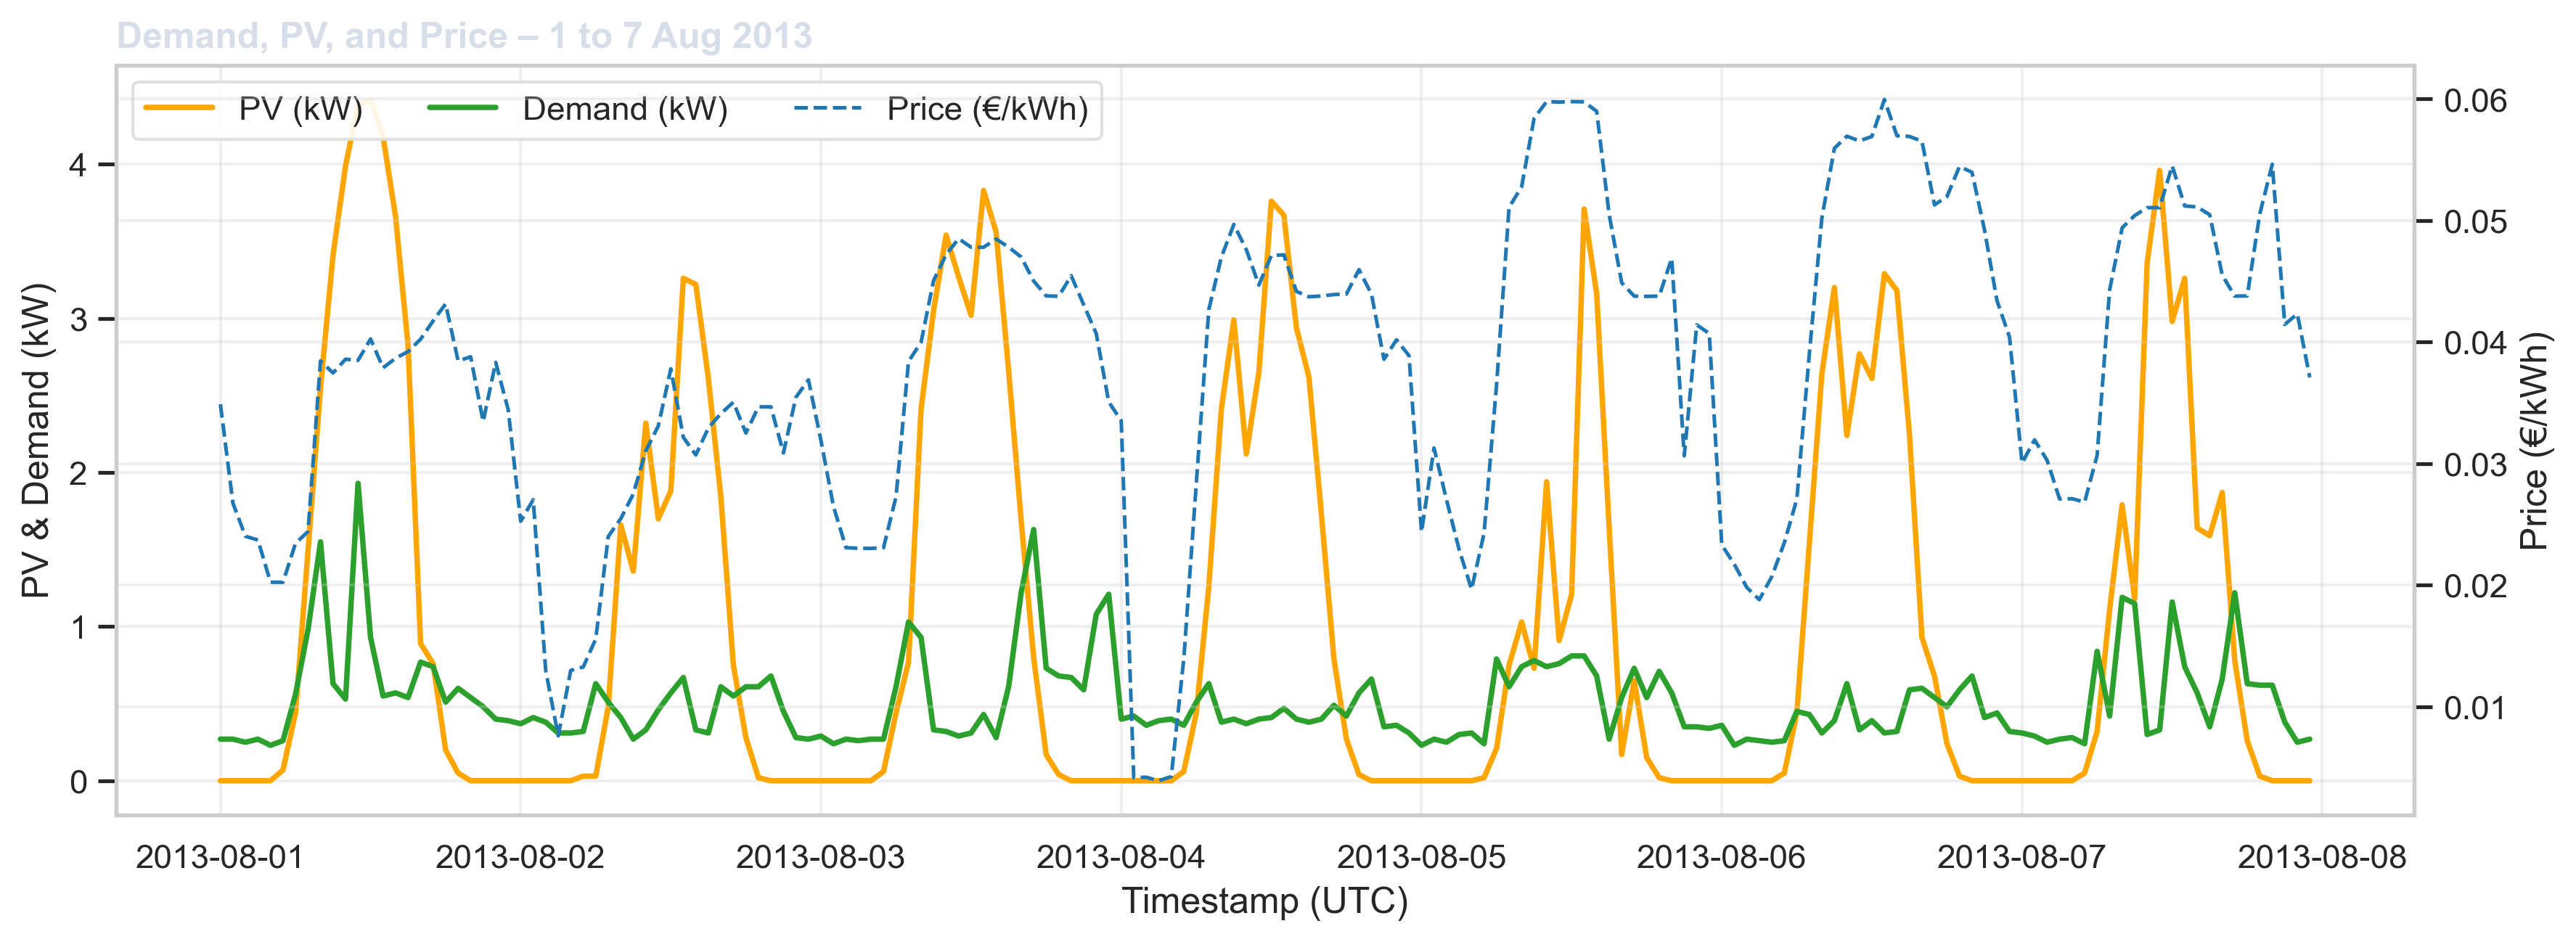
\includegraphics[width=\linewidth]{task3_fig1_timeseries_overlay.png}
  \caption{Time series overlay (Demand, PV, Price) over a representative week. PV peaks at midday while demand peaks appear in morning/evening; price co-moves with scarcity.}
  \label{fig:task3_ts_overlay}
\end{figure}

\begin{figure}[H]
  \centering
  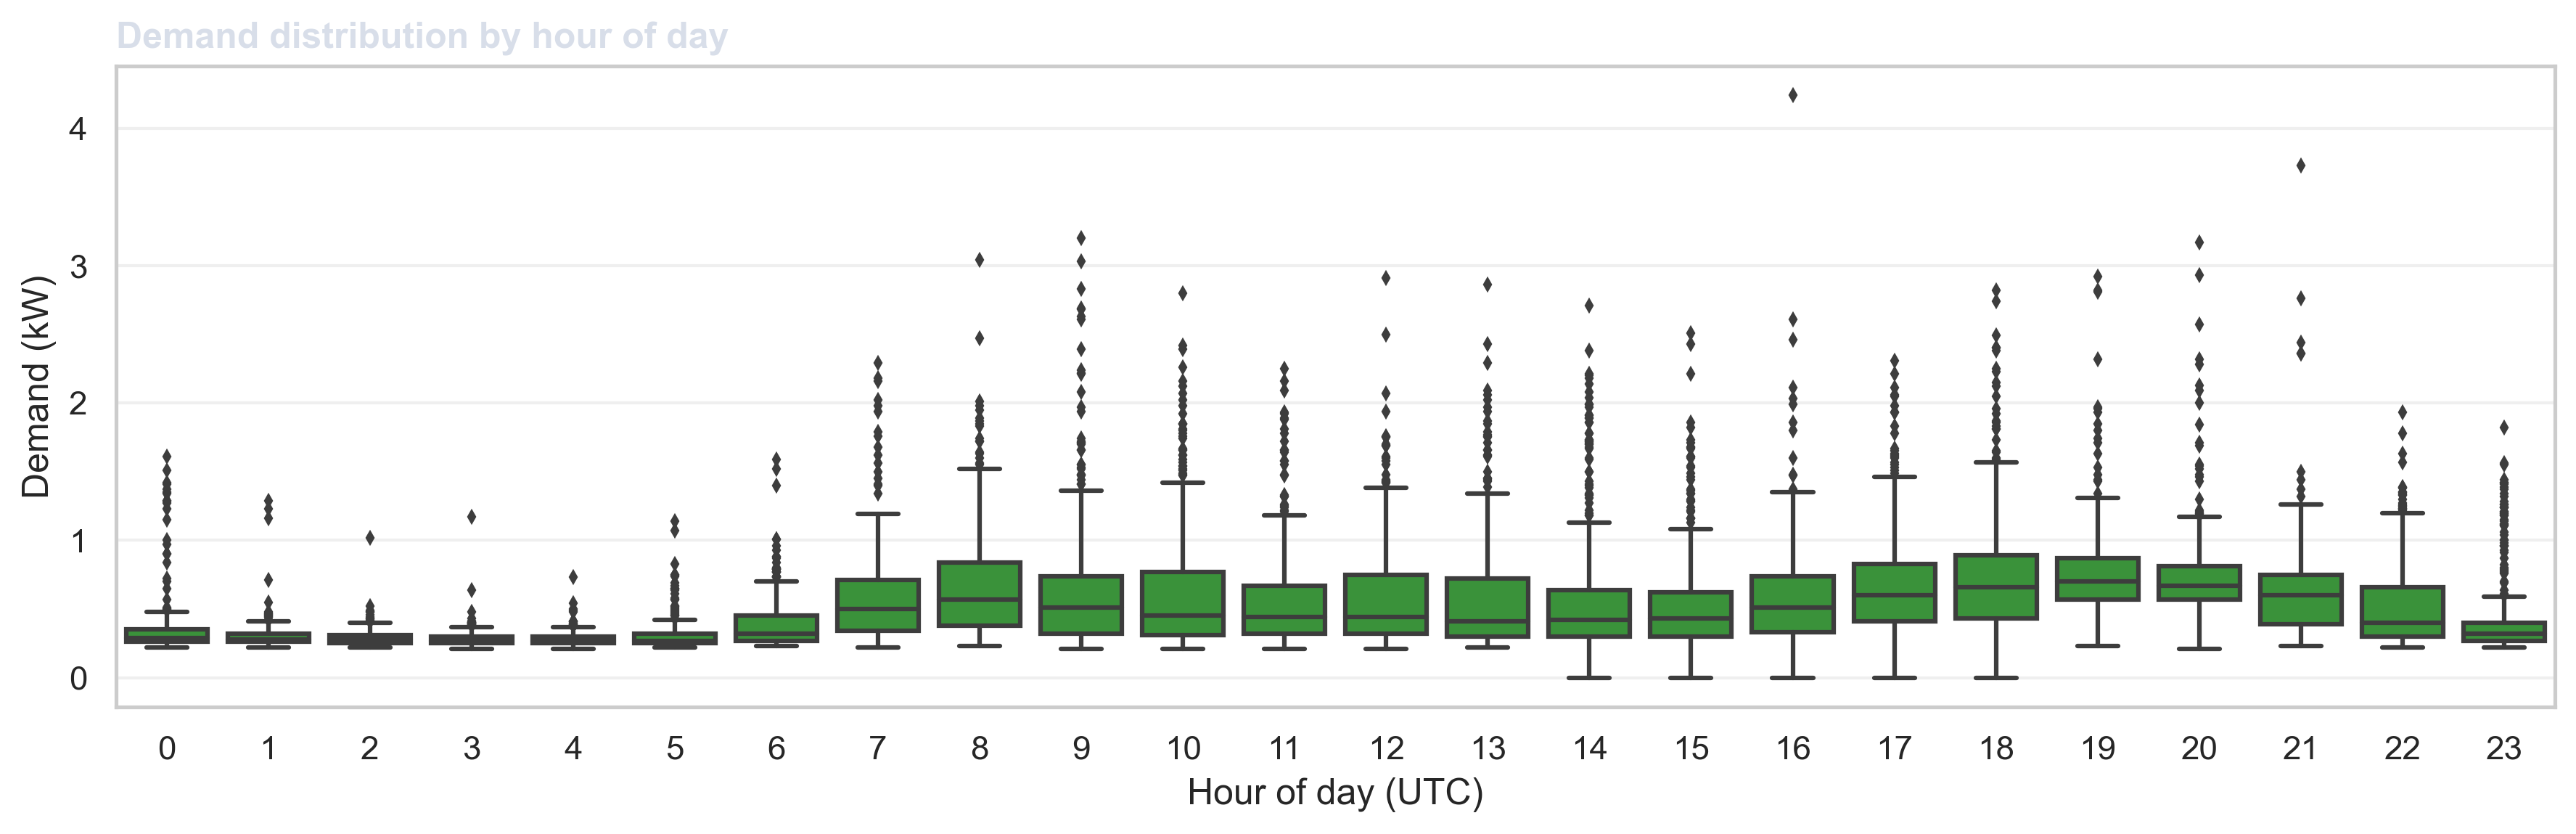
\includegraphics[width=0.9\linewidth]{task3_fig3_hourly_boxplot.png}
  \caption{Hourly demand boxplots highlighting diurnal variability and evening peaks relevant for storage dispatch.}
  \label{fig:task3_boxplots}
\end{figure}

\begin{figure}[H]
  \centering
  \includegraphics[width=0.95\linewidth]{task3_fig2_distributions.png}
  \caption{Histograms with KDE for Demand and PV showing typical operating ranges and skewness.}
  \label{fig:task3_histograms}
\end{figure}

\begin{figure}[H]
  \centering
  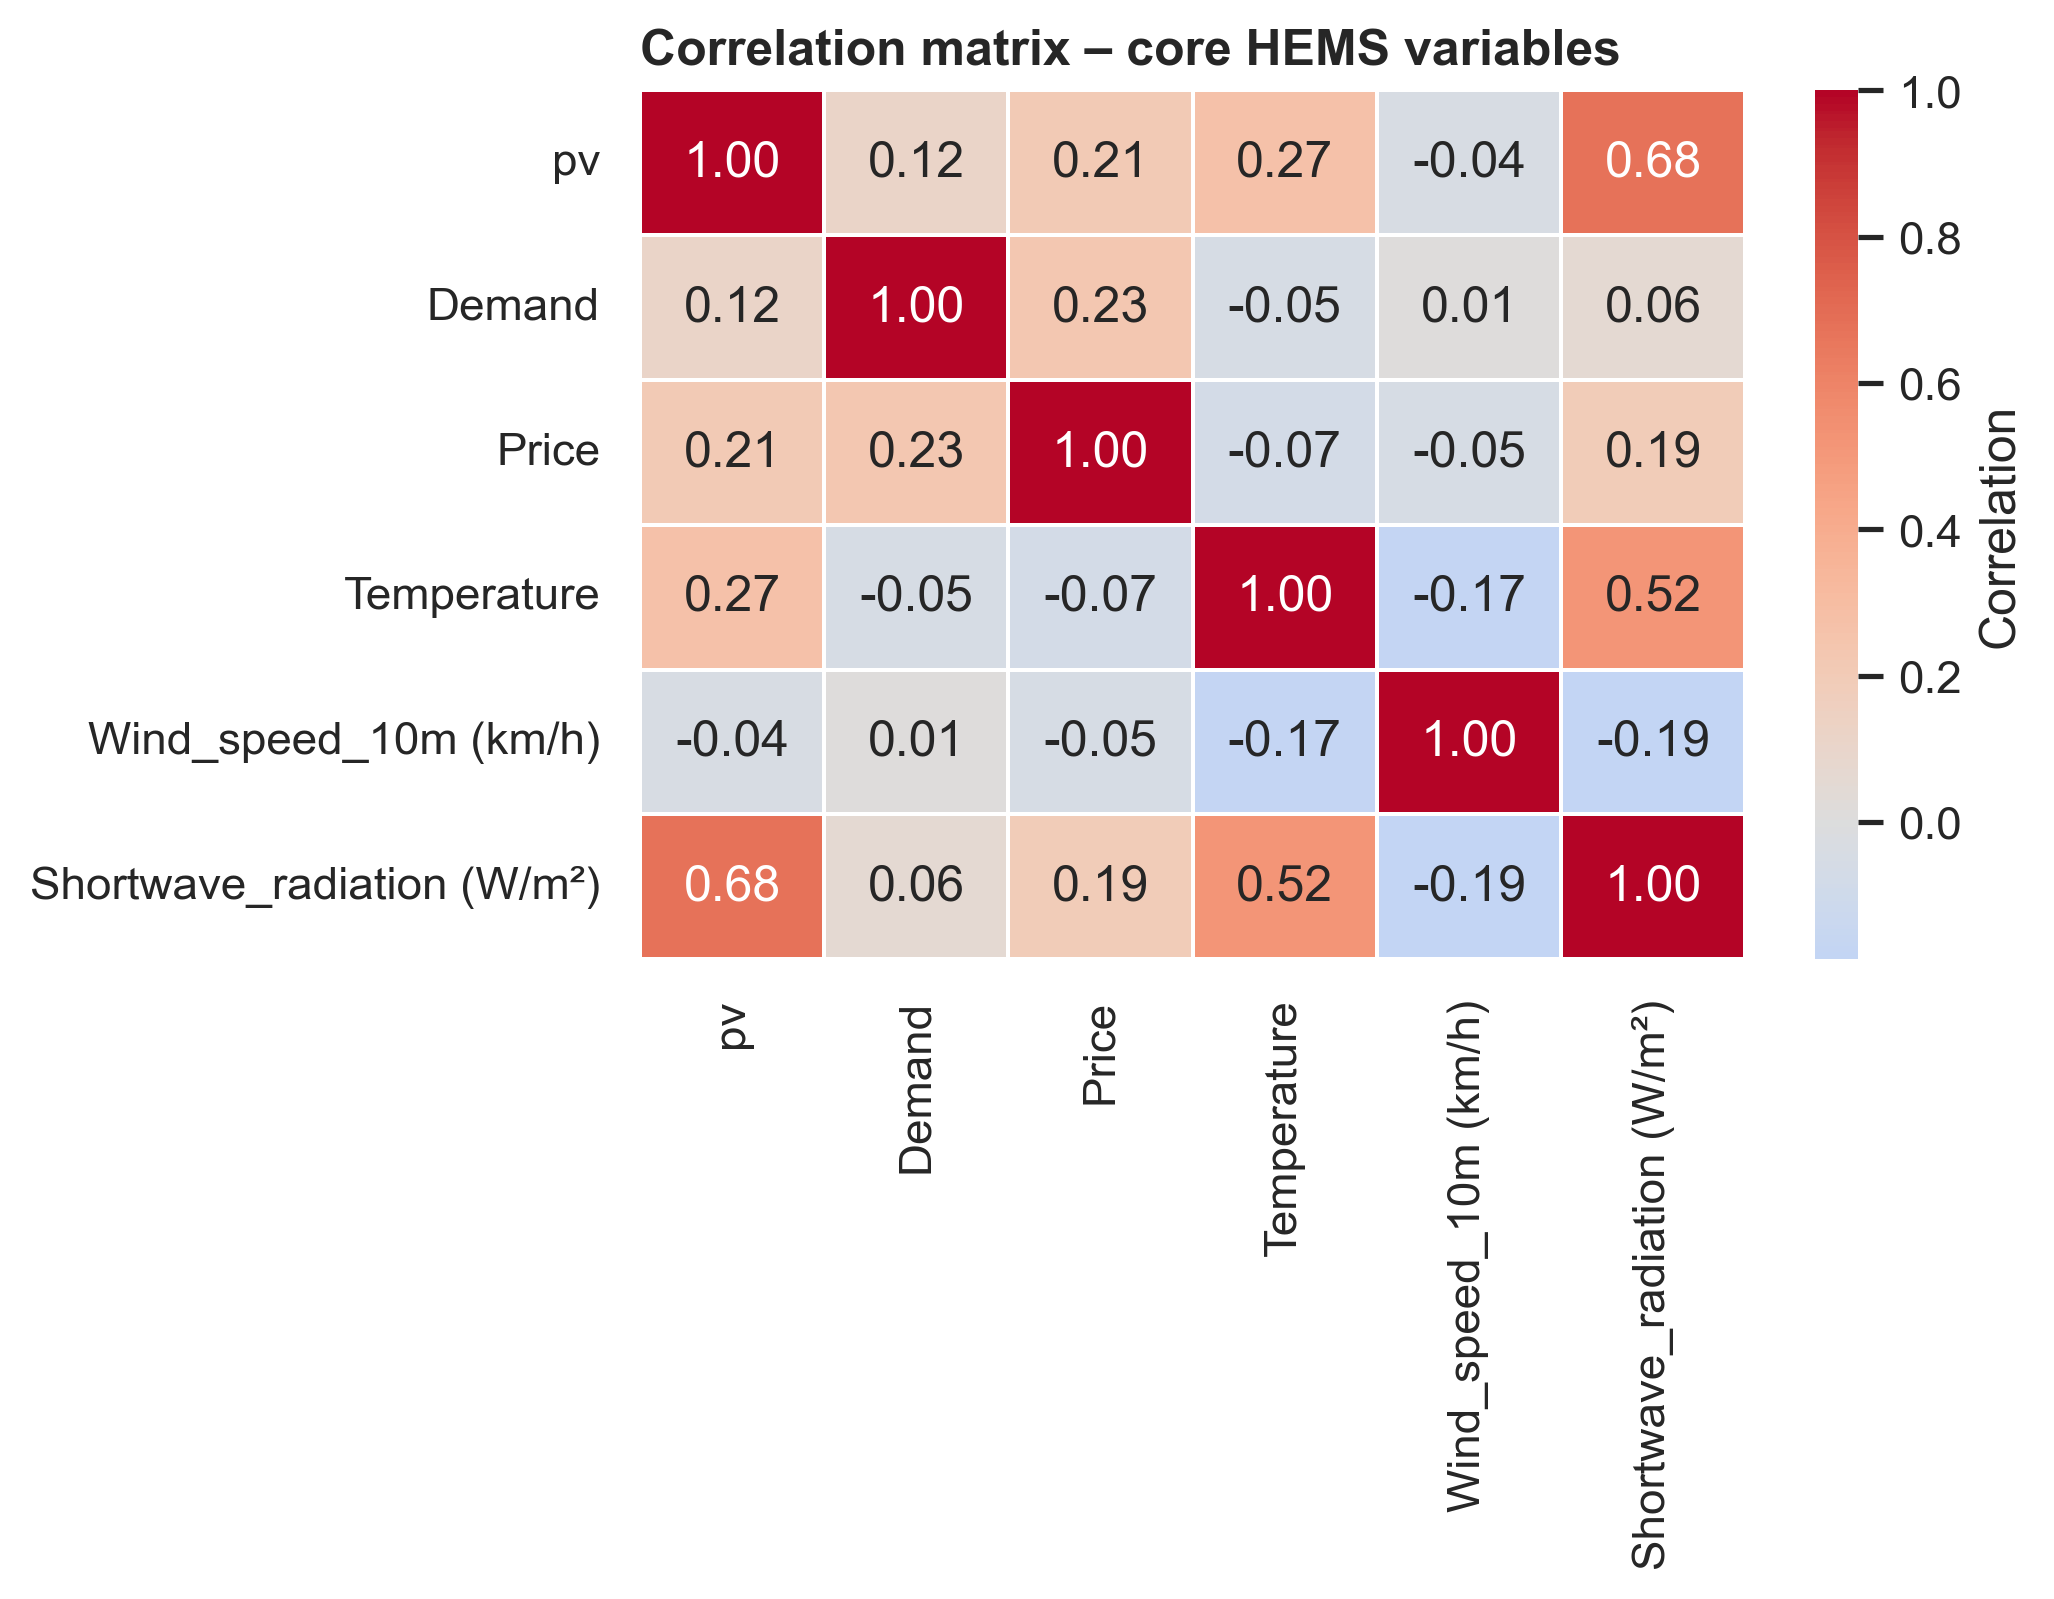
\includegraphics[width=0.8\linewidth]{task3_fig4_correlation_heatmap.png}
  \caption{Correlation heatmap for core variables: positive association between demand and price; midday PV is broadly anti-correlated with net demand.}
  \label{fig:task3_corr}
\end{figure}

\subsection{Interpretation and insights}
The figures reveal strong diurnal and weekday effects (peak demand in morning/evening; PV midday peaks). Correlation patterns motivate feature engineering: calendar variables (hour, weekday), weather covariates (irradiance, temperature), and lagged terms for persistence \cite{Hyndman2021}. Among the plots, the typical hourly structure captured by boxplots and profiles is most informative for downstream HEMS decisions because it concisely indicates when PV–demand mismatches are systematic and sizable, guiding storage control; these visuals adhere to ethical design (clear labels, units, non-deceptive axes) and maximize readability and completeness \cite{Antonanzas2016}.

%===========================
% 4. Data Cleaning
%===========================
\section*{4. Data cleaning}

\subsection*{4.1 Missingness profiling}
We begin with a systematic audit of missingness across the time series. Figure~\ref{fig:task4_missing_heatmap} visualises missing data over time and variables, while Table~\ref{tab:task4_missing_summary} summarises counts and rates. Patterns concentrated at specific periods (e.g., sensor outages) suggest Missing At Random (MAR), while isolated holes may be plausibly Missing Completely At Random (MCAR). When missingness depends on unobserved values (MNAR), simple imputations risk bias \cite{Little2002}.

\begin{figure}[H]
  \centering
  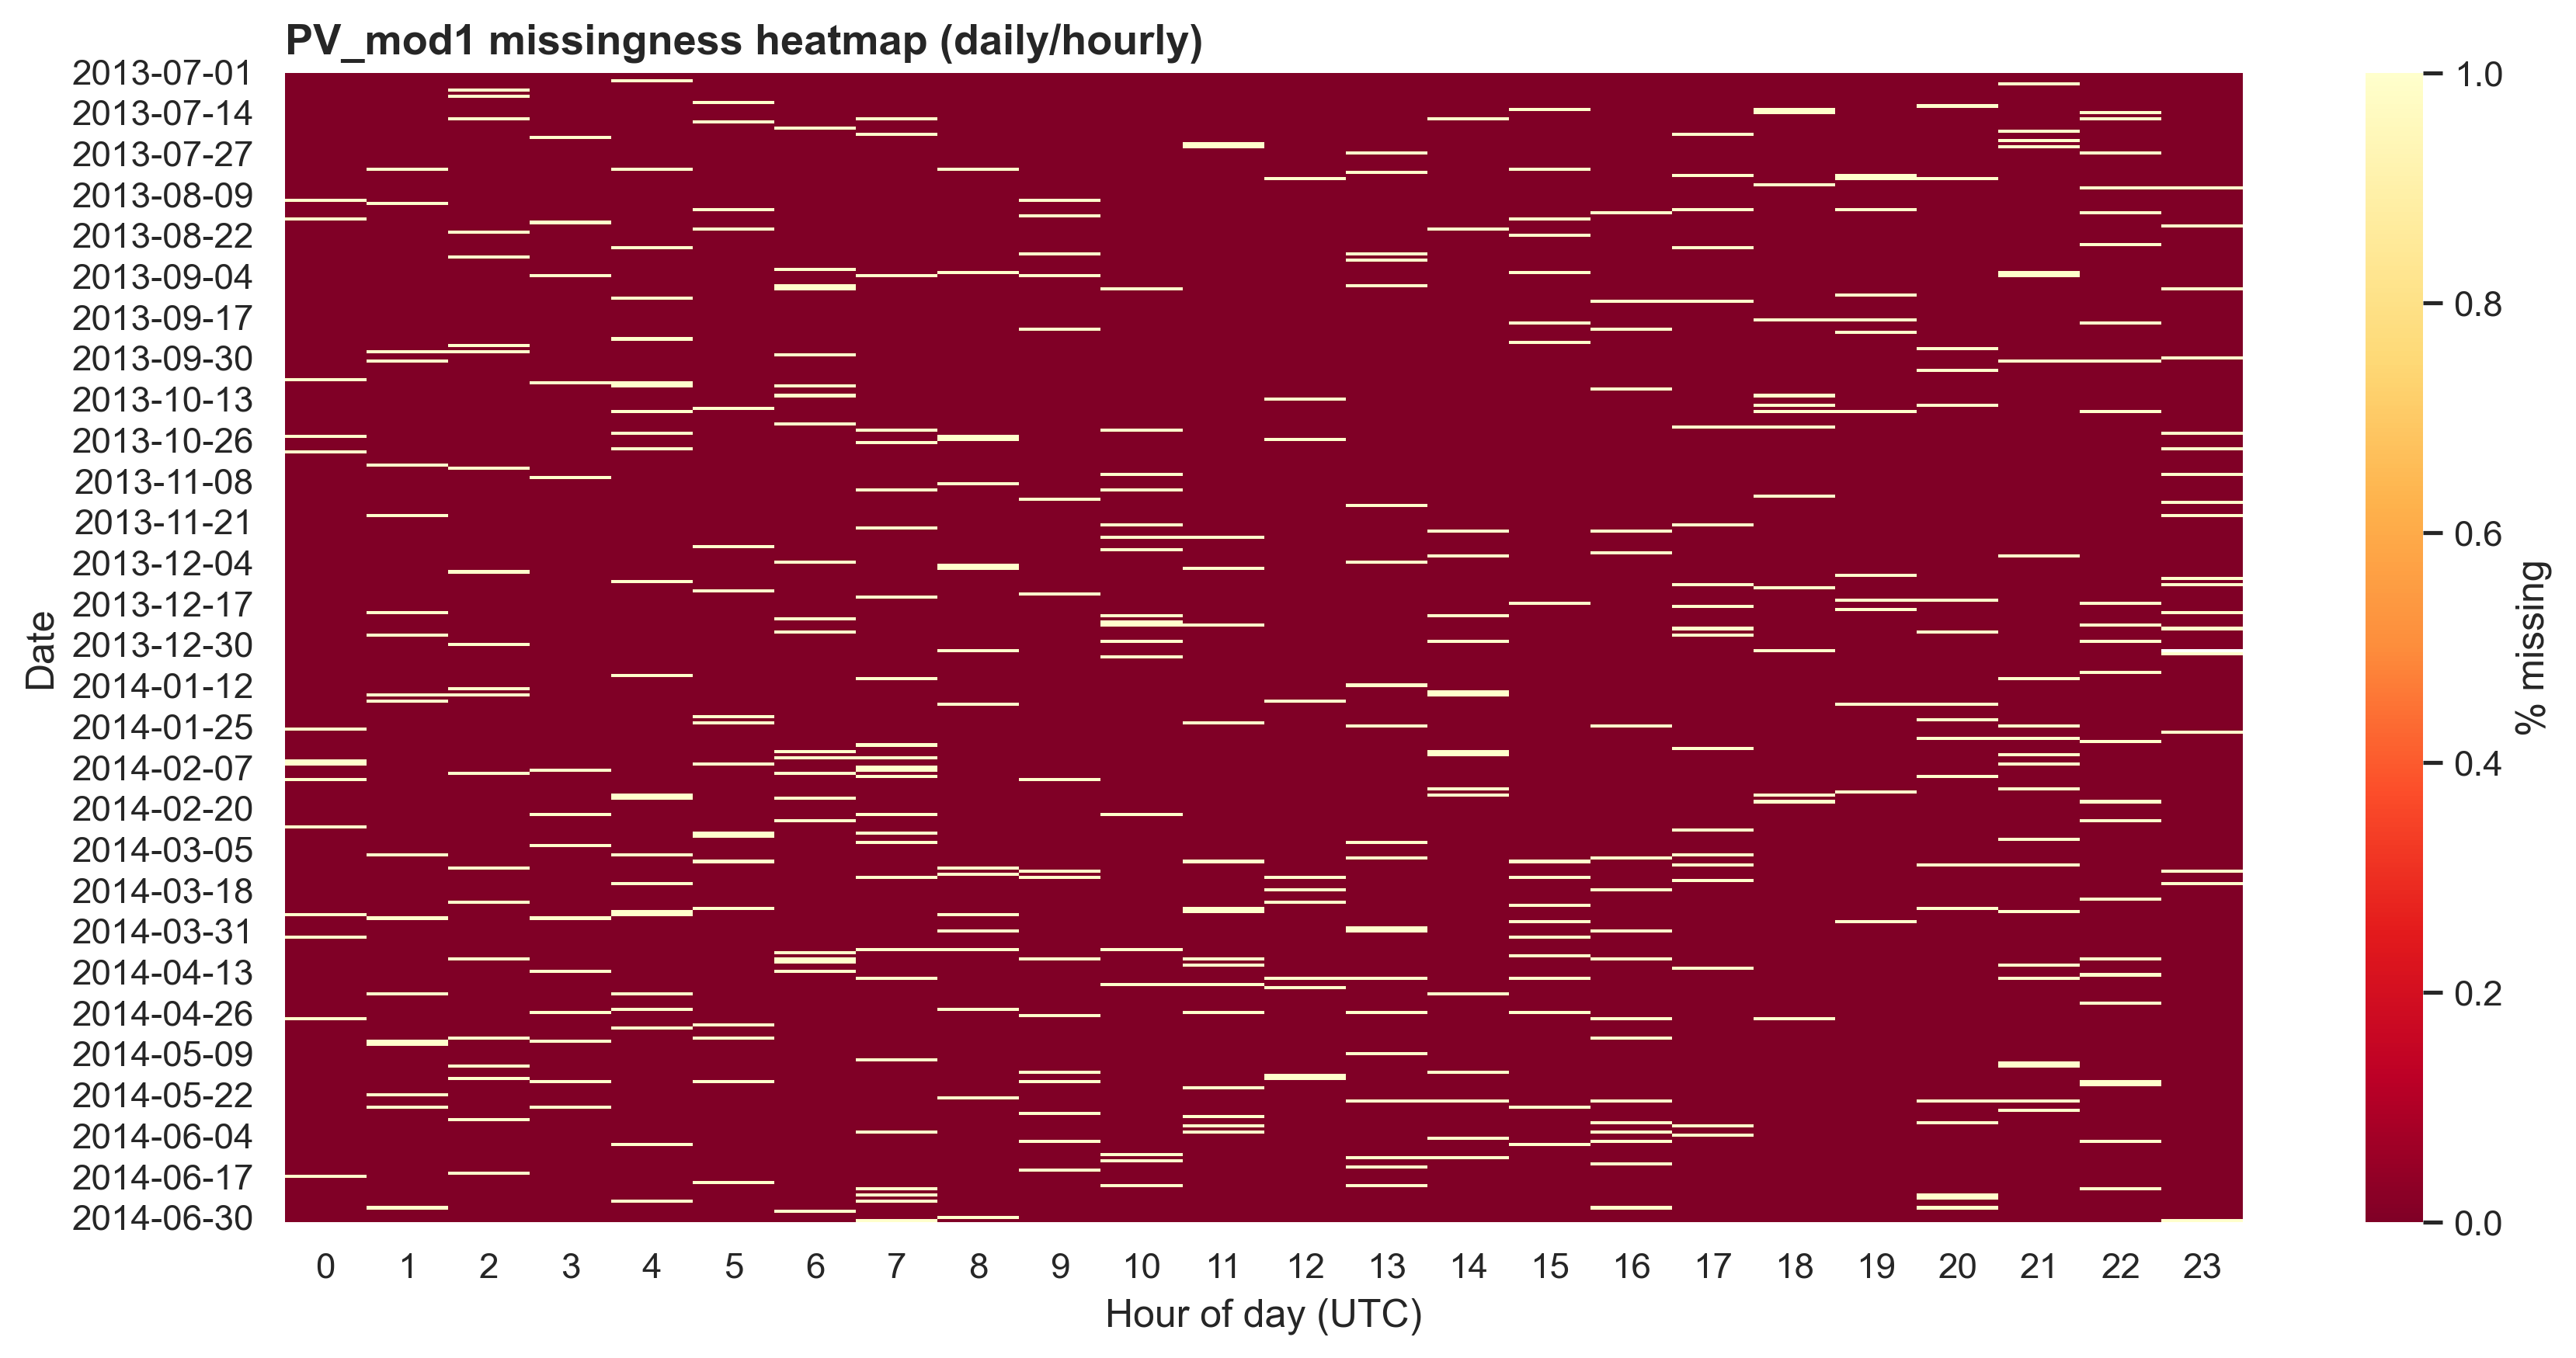
\includegraphics[width=0.95\linewidth]{task4_fig_missing_heatmap.png}
  \caption{Missingness heatmap across variables and time. Clusters indicate outages; isolated gaps may be random losses.}
  \label{fig:task4_missing_heatmap}
\end{figure}

\begin{table}[H]
  \centering
  \caption{Summary of missing values by variable and overall rate.}
  \label{tab:task4_missing_summary}
  \csvautobooktabular{tables/task4_missing_summary.csv}
\end{table}

\subsection*{4.2 Time-of-day and run-length diagnostics}
To detect structural gaps (e.g., firmware resets at fixed hours), we examine missingness by hour-of-day and contiguous run lengths. Figure~\ref{fig:task4_missing_tod} shows missing rate by hour; Table~\ref{tab:task4_missing_tod_tbl} lists per-hour rates. A timeline view (Figure~\ref{fig:task4_missing_timeline}) highlights multi-hour runs that merit careful treatment (e.g., forward-fill caps) rather than naive interpolation.

\begin{figure}[H]
  \centering
  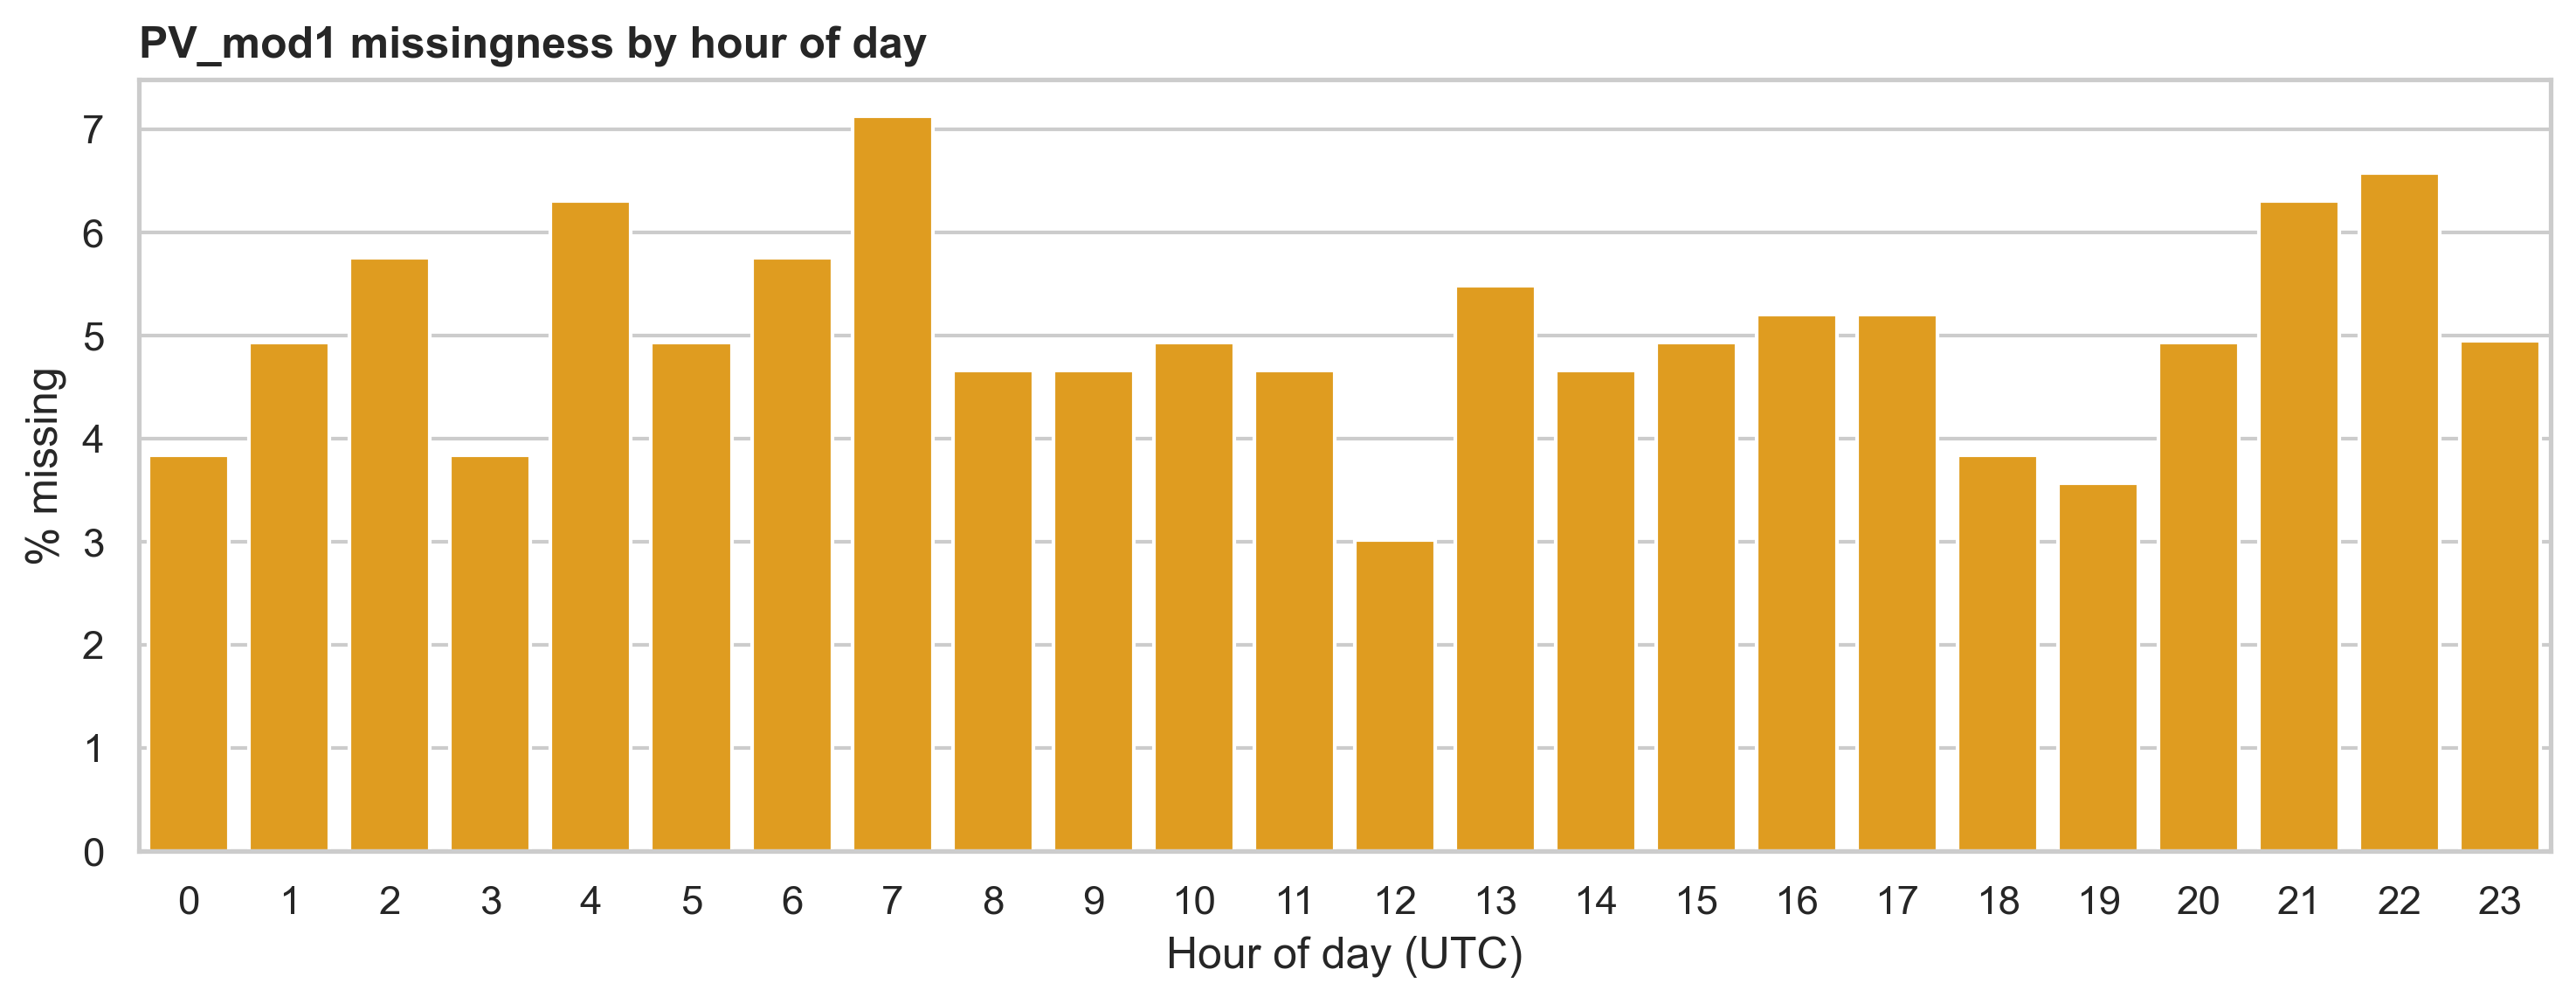
\includegraphics[width=0.8\linewidth]{task4_fig_missing_tod.png}
  \caption{Missingness by hour-of-day (share of samples missing).}
  \label{fig:task4_missing_tod}
\end{figure}

\begin{table}[H]
  \centering
  \caption{Hourly missingness rates.}
  \label{tab:task4_missing_tod_tbl}
  \csvautobooktabular{tables/task4_missing_tod.csv}
\end{table}

\begin{figure}[H]
  \centering
  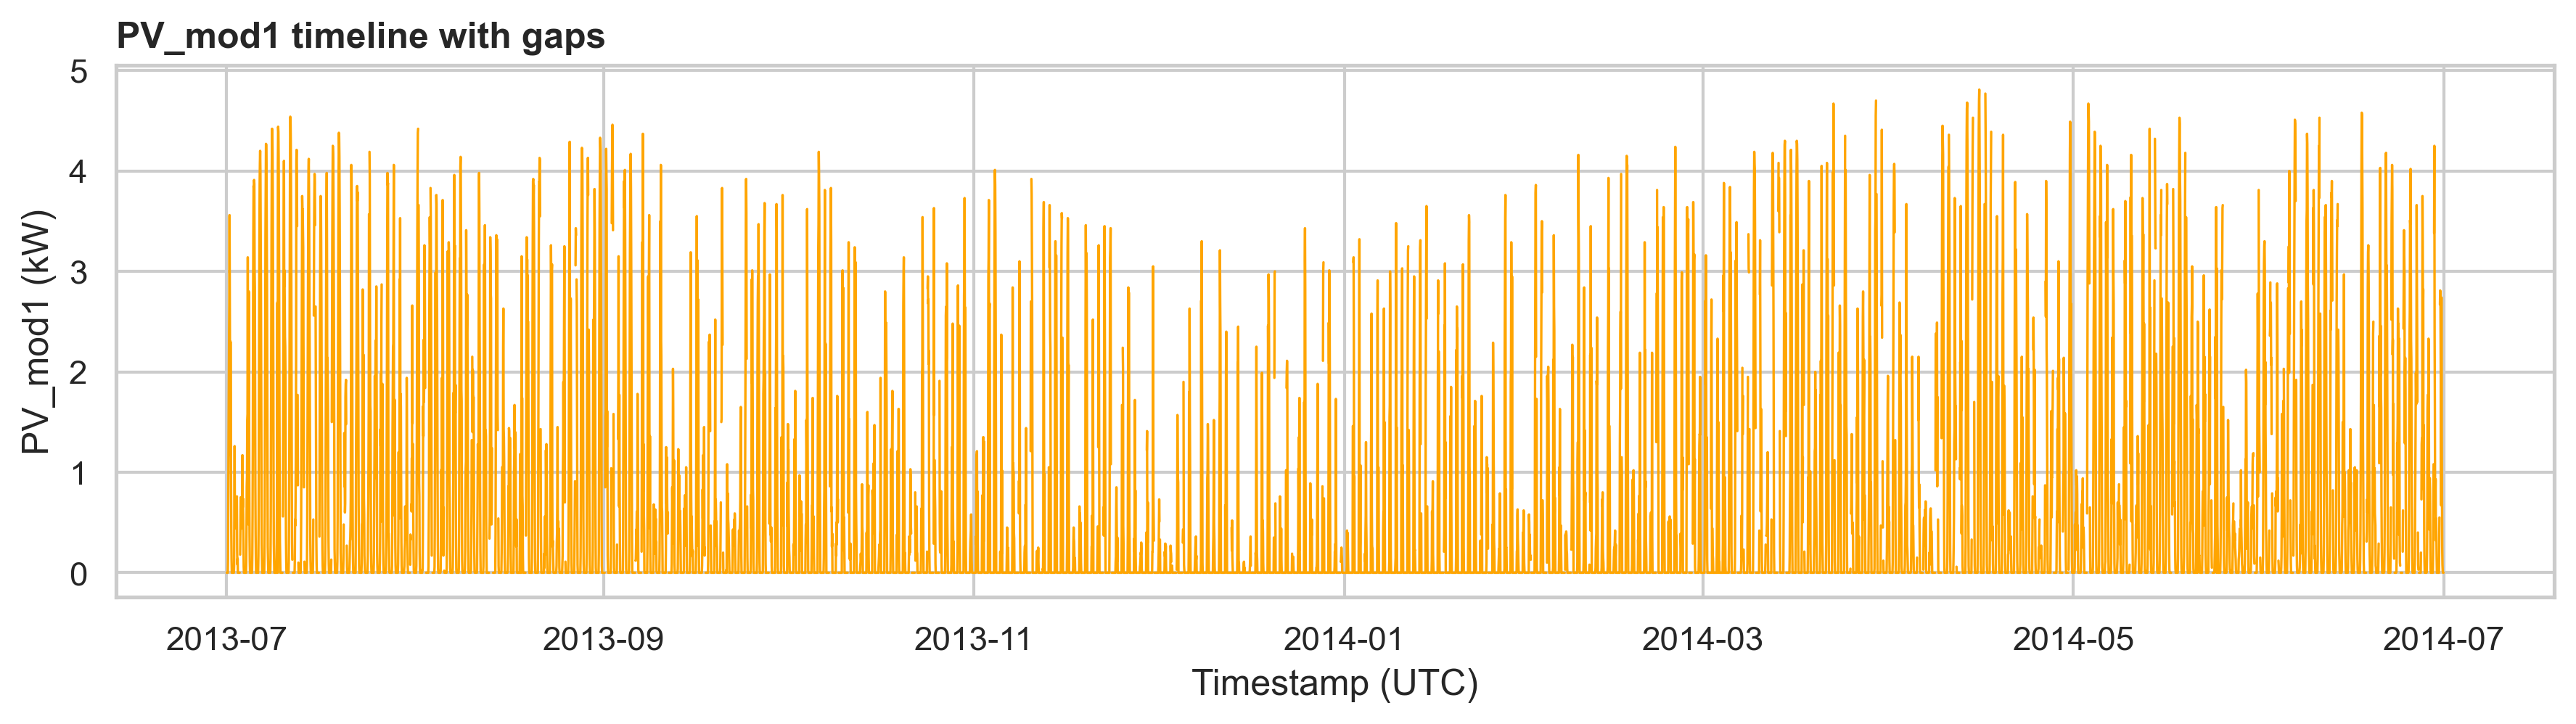
\includegraphics[width=0.95\linewidth]{task4_fig_missing_timeline.png}
  \caption{Timeline view of missingness runs, revealing outage episodes.}
  \label{fig:task4_missing_timeline}
\end{figure}

\subsection*{4.3 Imputation strategy and validation}
Given the strong daily structure, we combine conservative forward/backward fills for short gaps with calendar-aware interpolation and, where suitable, model-based imputation using seasonally adjusted series. Figure~\ref{fig:task4_imputation_overlay} overlays raw and imputed series for a representative window; Table~\ref{tab:task4_imputation_summary} reports diagnostic metrics (e.g., gap length distribution, post-imputation variance preservation). We avoid imputing PV at night (kept at zero) and cap fills over long runs to prevent artificial smoothing \cite{Hyndman2021,Little2002}.

\begin{figure}[H]
  \centering
  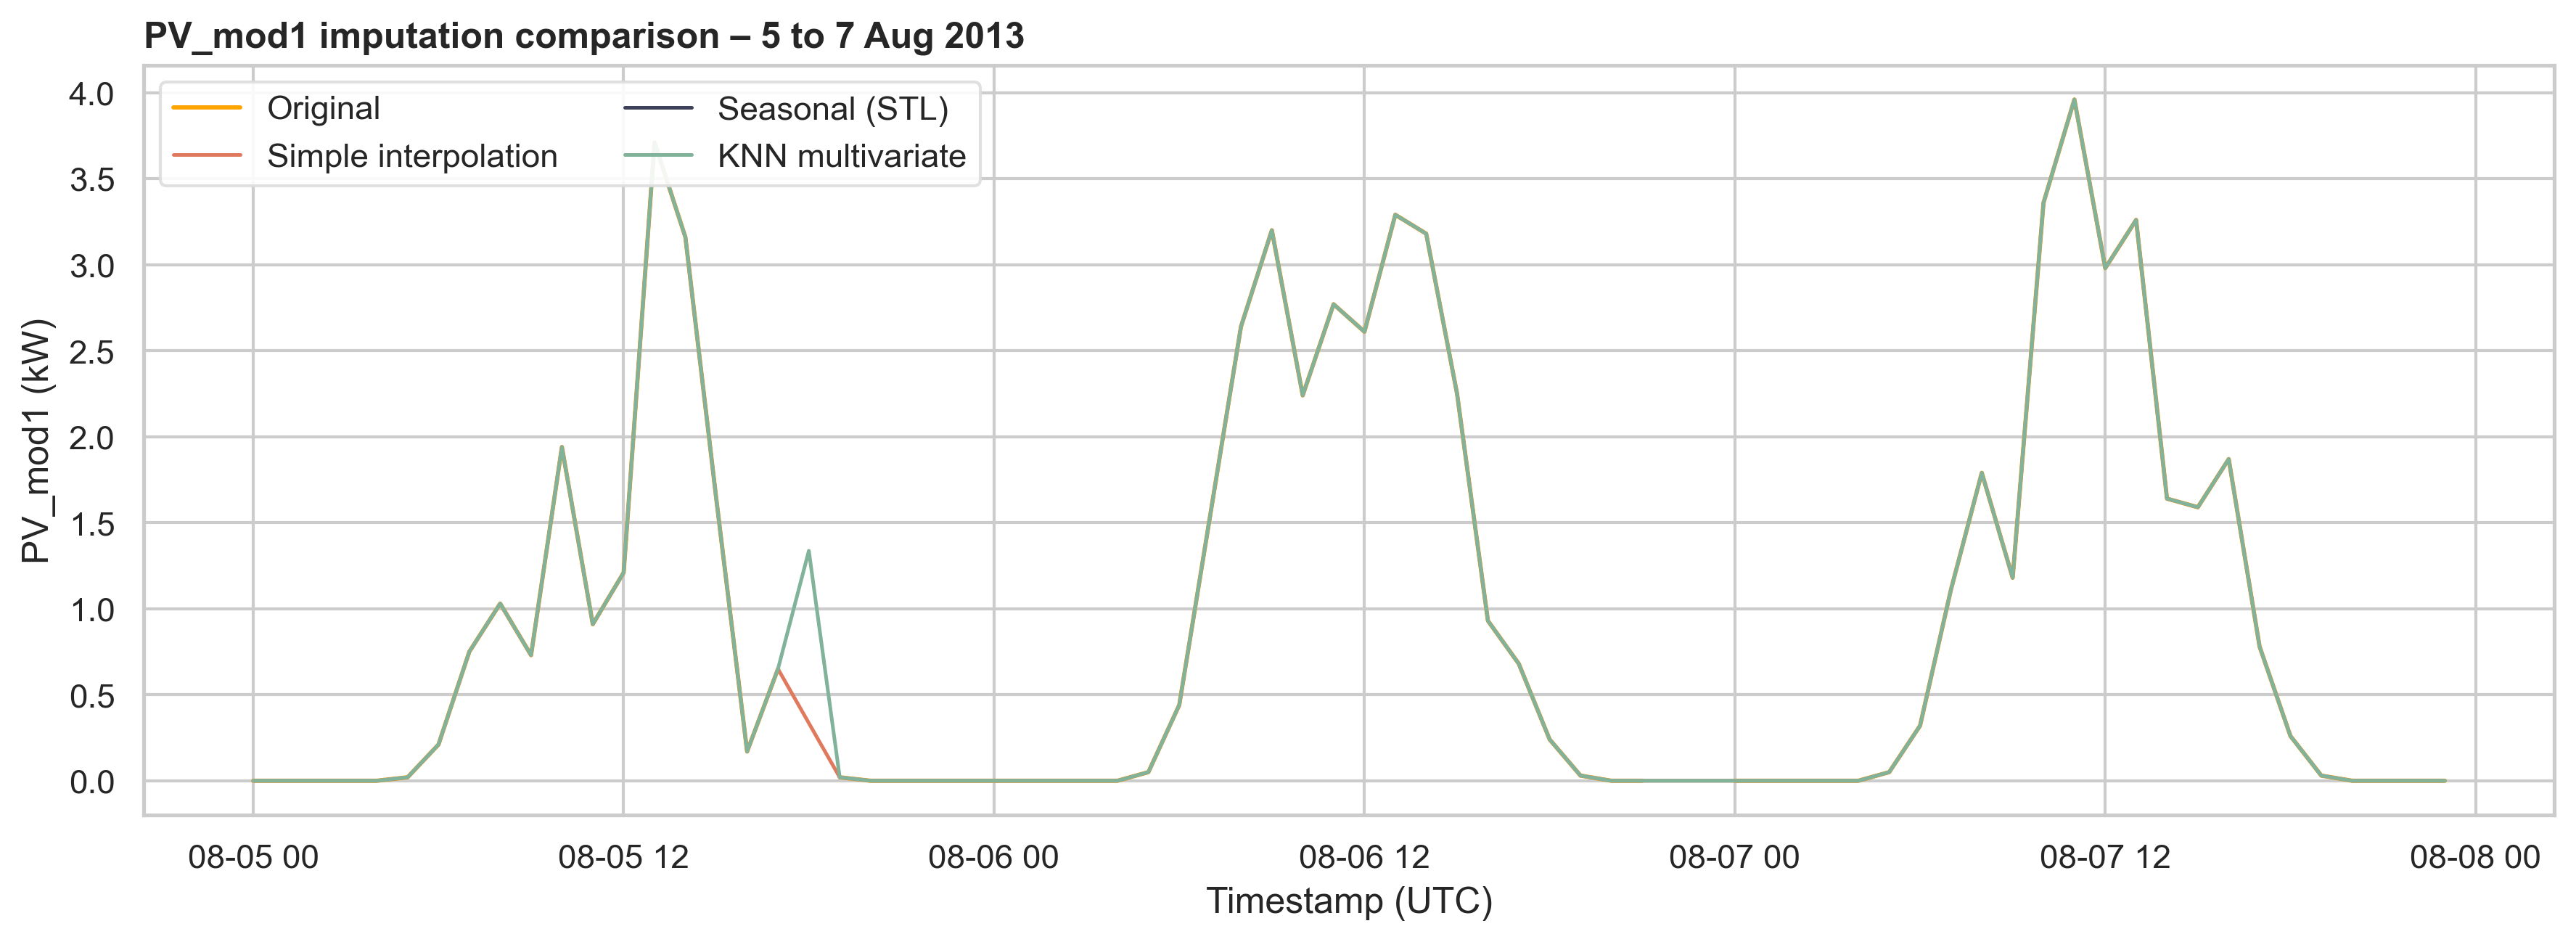
\includegraphics[width=0.95\linewidth]{task4_fig_imputation_overlay.png}
  \caption{Imputation overlay: raw versus imputations across typical gaps. Strategy preserves diurnal shape while preventing drift.}
  \label{fig:task4_imputation_overlay}
\end{figure}

\begin{table}[H]
  \centering
  \caption{Imputation diagnostics summary.}
  \label{tab:task4_imputation_summary}
  \csvautobooktabular{tables/task4_imputation_summary.csv}
\end{table}

\subsection*{4.4 Seasonal decomposition as a diagnostic}
Seasonal-Trend decomposition (STL) helps verify that cleaning preserves essential structure. Figure~\ref{fig:task4_stl} shows clean series decomposed into trend, seasonal, and remainder. Seasonal amplitude and stable remainder suggest that imputations did not introduce artifacts and that later ARIMA/ML models can exploit clear seasonality \cite{Hyndman2021}.

\begin{figure}[H]
  \centering
  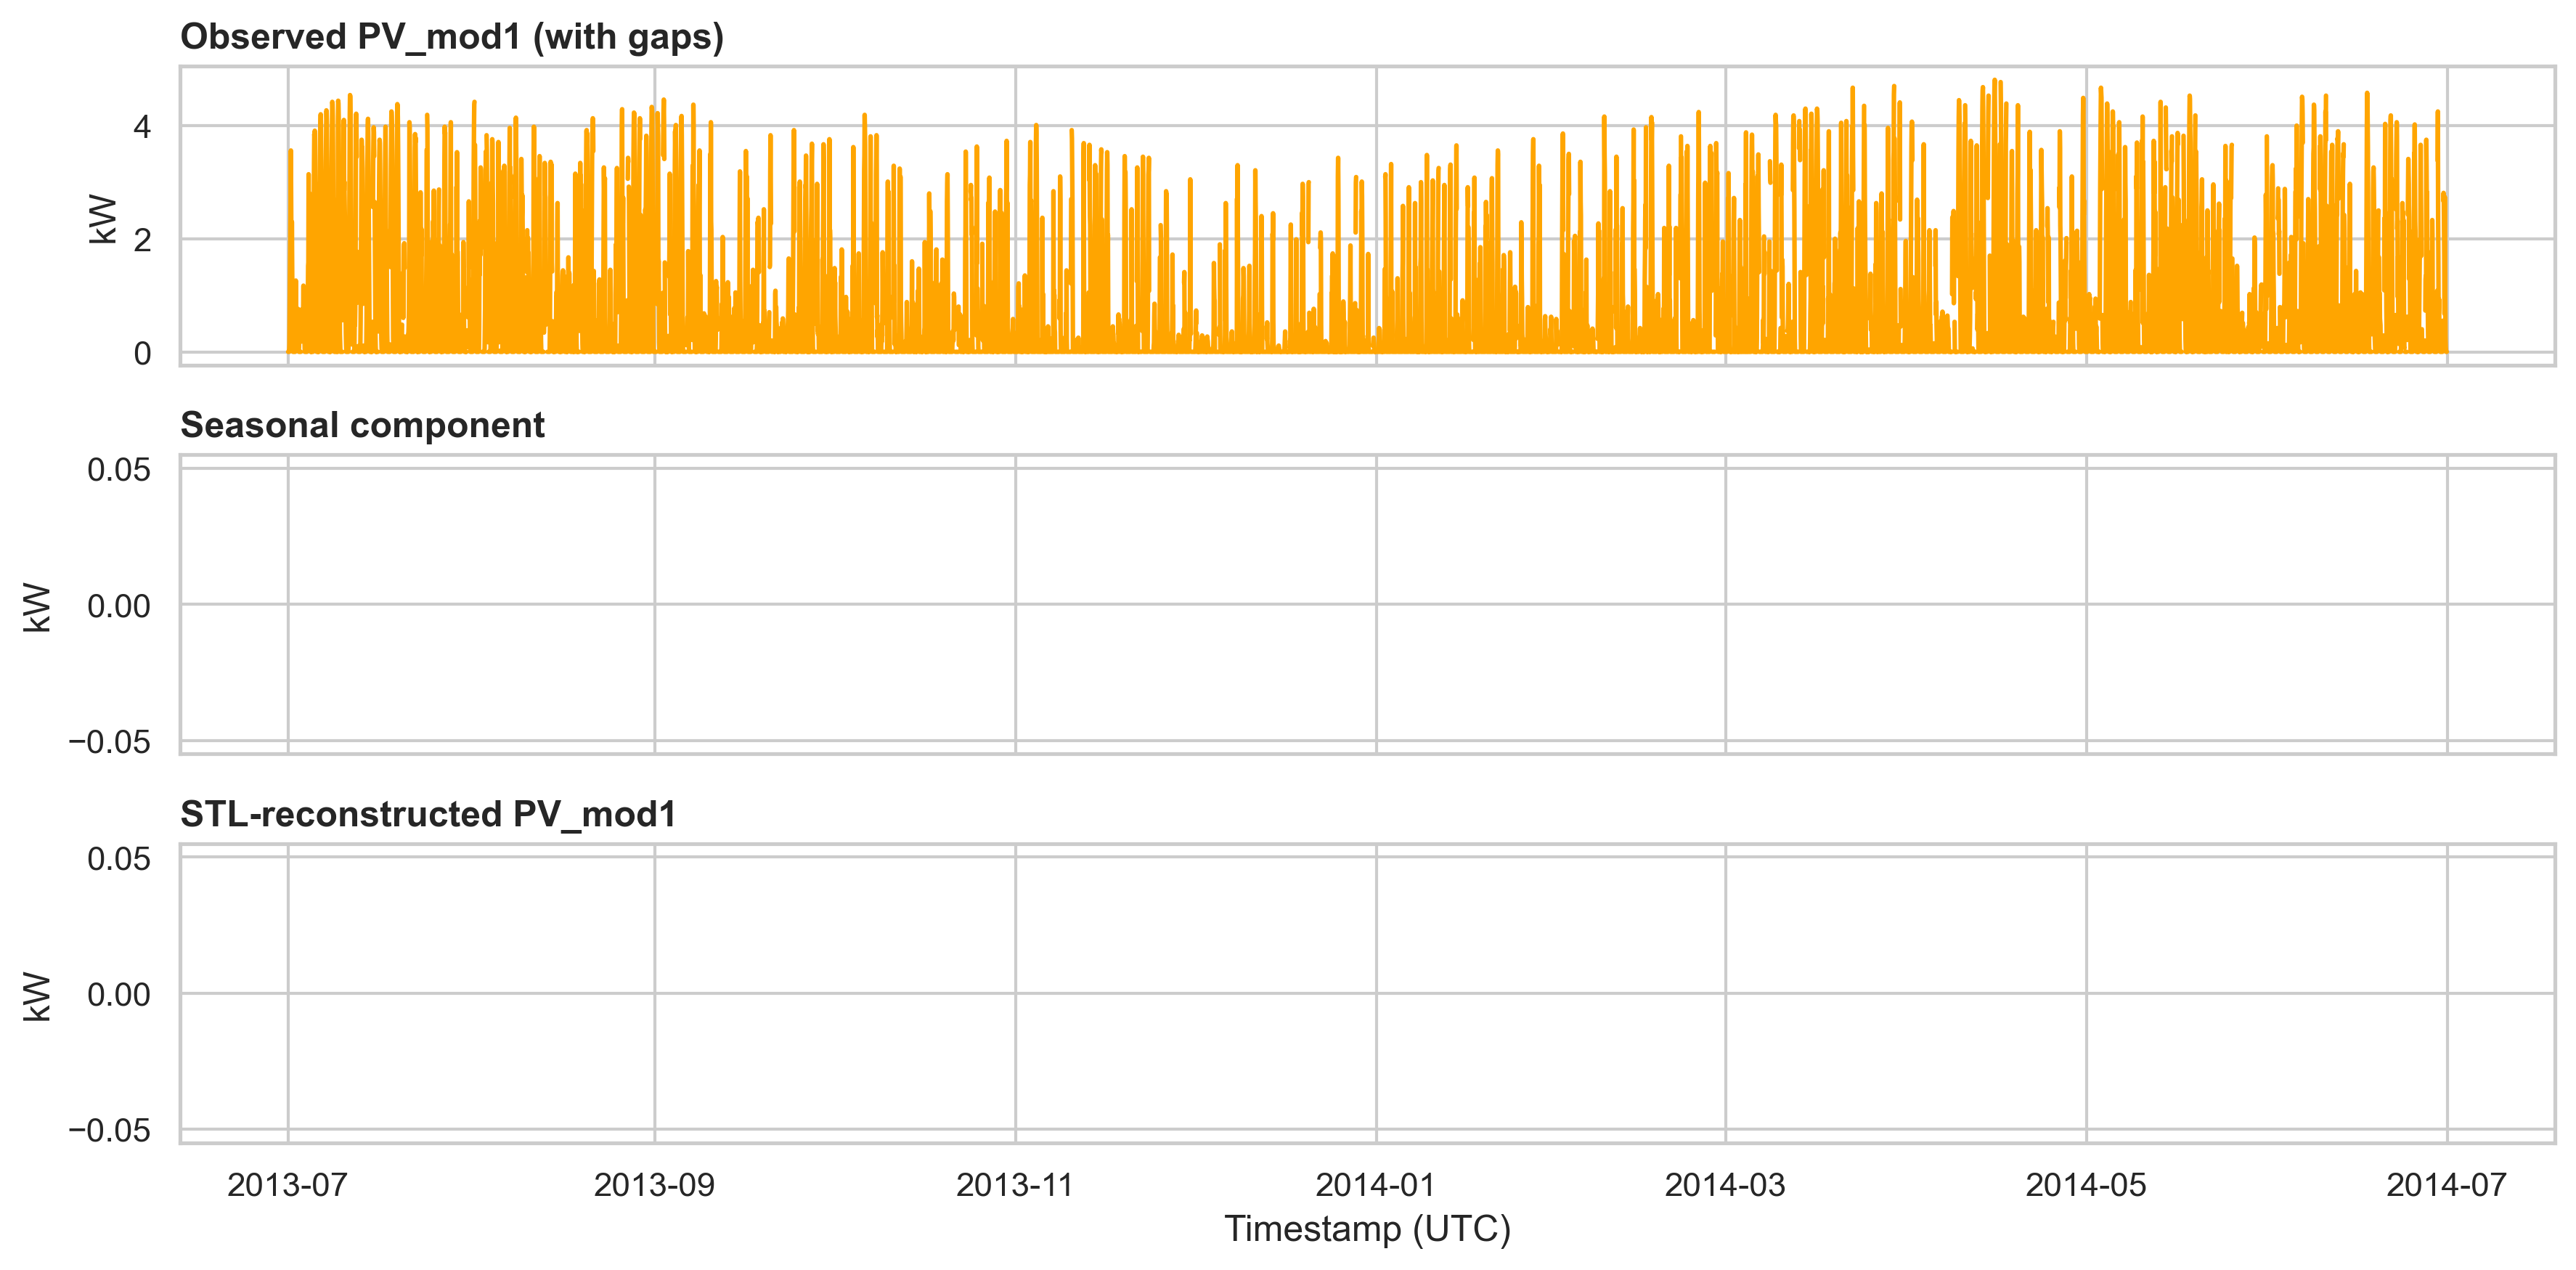
\includegraphics[width=0.95\linewidth]{task4_fig_stl_components.png}
  \caption{STL components after cleaning: strong diurnal seasonality with reasonable remainder variance.}
  \label{fig:task4_stl}
\end{figure}

\subsection*{4.5 Daily profiles before and after cleaning}
To verify that imputations did not distort operational patterns, we compare typical daily profiles. Figure~\ref{fig:task4_daily_profiles} indicates that peak timings and amplitudes remain consistent, while extreme outliers are mitigated—desirable for forecasting stability and optimisation downstream.

\begin{figure}[H]
  \centering
  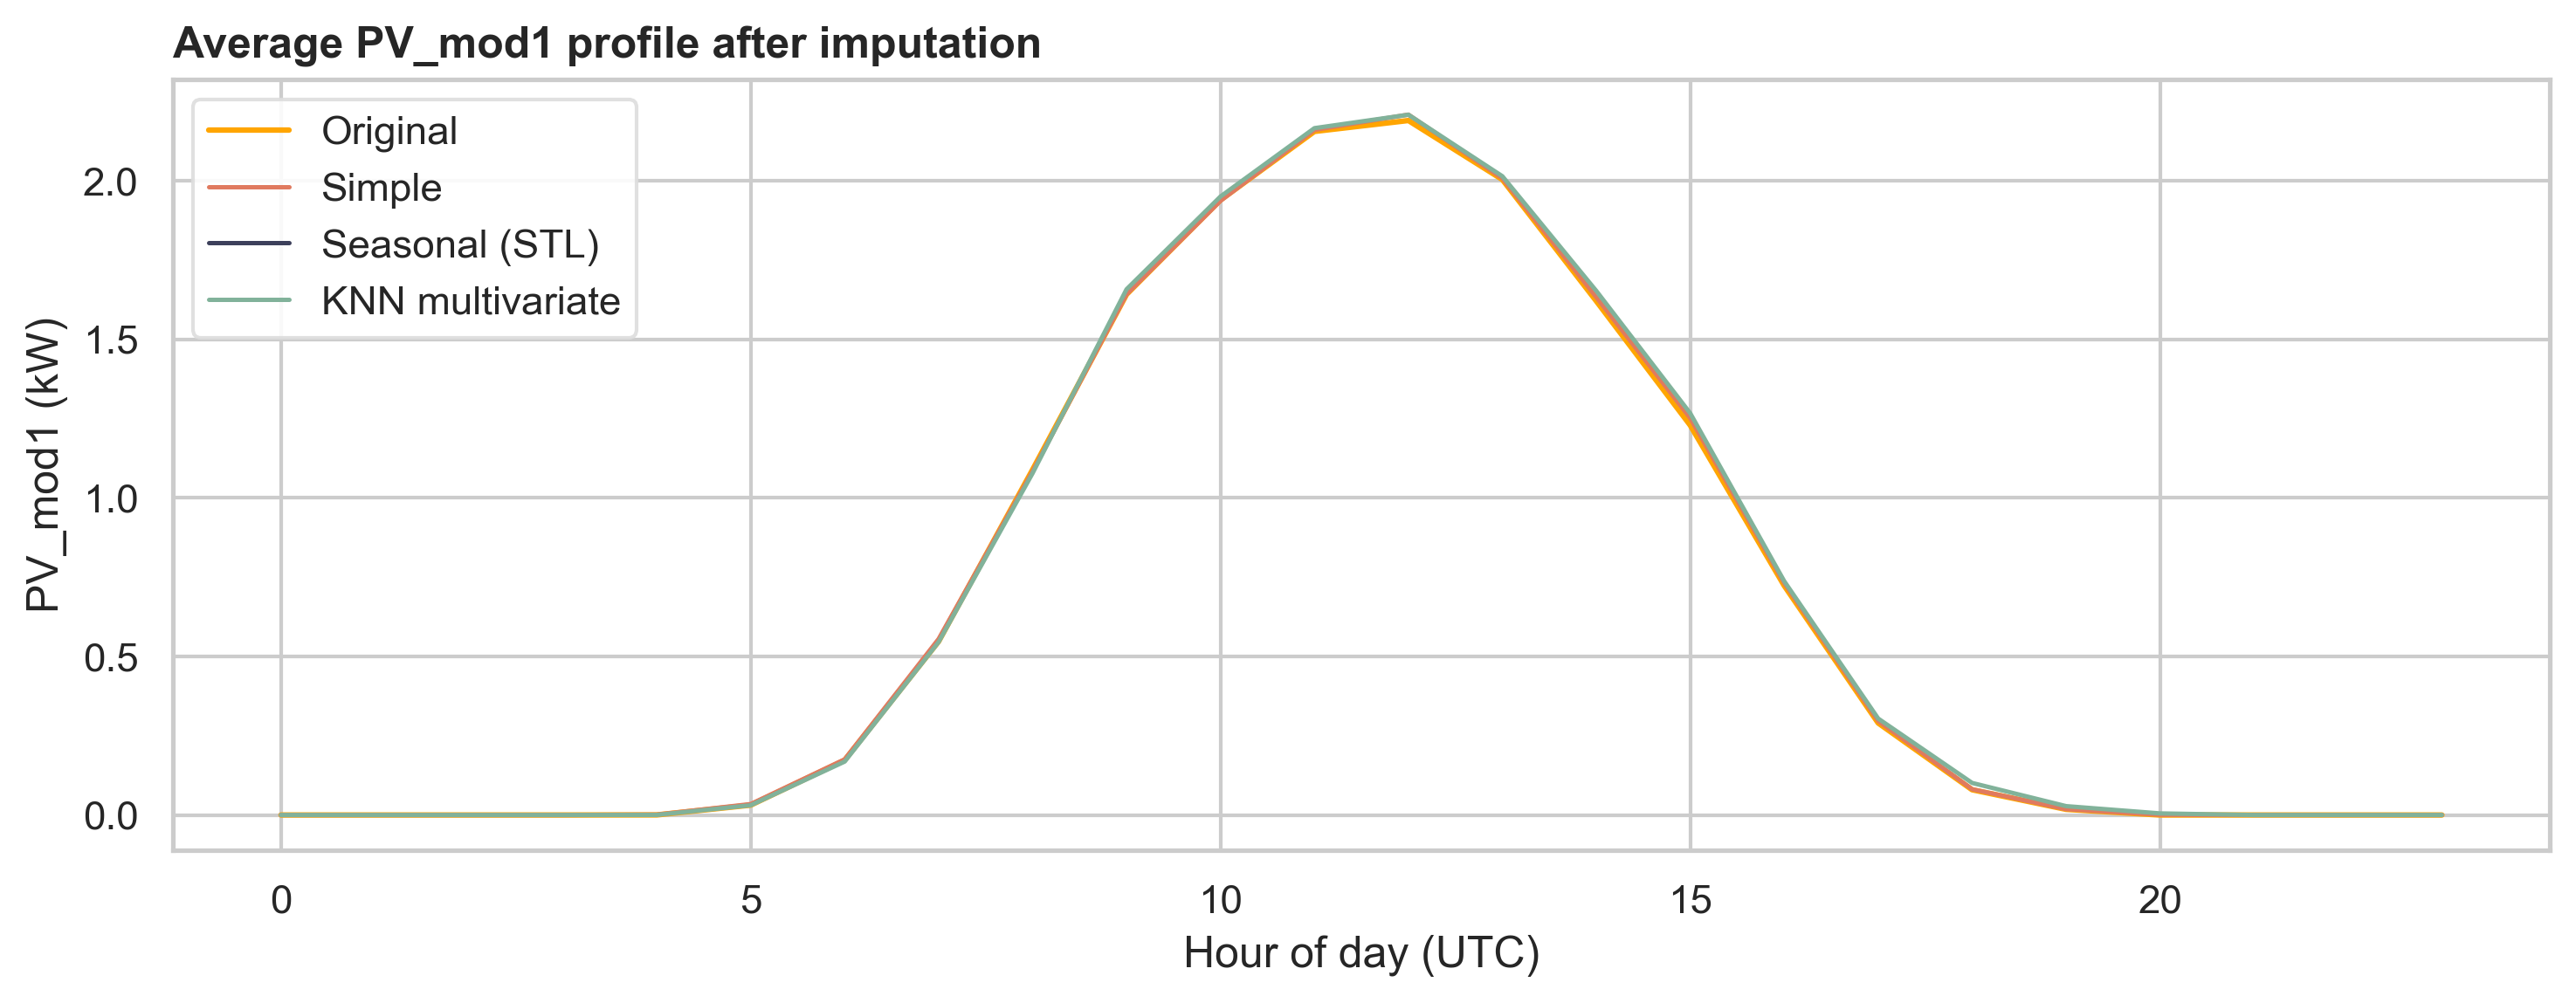
\includegraphics[width=0.9\linewidth]{task4_fig_daily_profiles.png}
  \caption{Typical daily profiles before/after cleaning for demand and PV (median and IQR).}
  \label{fig:task4_daily_profiles}
\end{figure}

\subsection*{4.6 Limitations and ethical considerations}
While the adopted imputation strategy is conservative, any gap-filling may obscure rare but important behaviours (e.g., extreme peaks). We therefore retain an audit trail of imputed indices and exclude heavily imputed windows from model validation to prevent optimistic bias. From an ethics perspective, cleaning steps avoid fabricating PV at night and preserve physical plausibility. Decisions are documented for reproducibility and to facilitate stakeholder scrutiny \cite{Little2002,Hyndman2021}.

\bigskip

	extbf{Outcome.} The cleaned dataset exhibits stable seasonal structure, reasonable variance, and documented imputations, forming a reliable basis for feature engineering (Task~5) and forecasting (Tasks~7--10).

%===========================
% 5. Feature engineering
%===========================
\section*{5. Feature engineering}

\subsection*{5.1 Objective and overview}
Feature engineering is central to improving predictive performance in short-term demand forecasting. By representing domain structure explicitly---diurnal and weekly cycles, weather sensitivity, persistence---we increase the signal-to-noise ratio that models can exploit \cite{Zheng2020,Hyndman2021}. We leverage three information streams: (i) the demand series (autoregressive lags and rolling summaries), (ii) weather covariates (temperature, solar radiation as proxy for PV), and (iii) calendar variables (hour-of-day, weekday/weekend, month, holidays).

\subsection*{5.2 Exploratory statistics}
We examine marginal distributions and bivariate relationships to motivate transformations and interactions.

\begin{figure}[H]
  \centering
  \includegraphics[width=0.95\linewidth]{figures/task3_fig2_distributions.png}
  \caption{Histograms with KDE for demand and temperature. Demand shows right-skew due to evening peaks; temperature is often closer to unimodal but may be seasonally shifted.}
  \label{fig:fe_hist_kde}
\end{figure}

\begin{figure}[H]
  \centering
  \includegraphics[width=0.9\linewidth]{figures/03_correlation_heatmap.png}
  \caption{Correlation snapshot among demand, temperature, PV/solar proxies, and price. Temperature typically correlates with demand (heating/cooling), while PV is anti-correlated with net demand at midday.}
  \label{fig:fe_corr}
\end{figure}

\begin{figure}[H]
  \centering
  \includegraphics[width=0.9\linewidth]{figures/03_overlay_demand_pv_price.png}
  \caption{Overlay of demand, PV and price illustrating alignment of peaks and troughs across drivers.}
  \label{fig:fe_overlay}
\end{figure}

Normalit{"a}t: Shapiro--Wilk-Tests auf stichprobenweise Fenster deuten bei Demand h{"a}ufig auf Nicht-Normalit{"a}t (p\,<\,0.05). Zur Stabilisierung der Varianz sind logarithmische oder Box--Cox-Transformationen geeignet, wobei f{"u}r Demand eine shift-Log (nur f{"u}r strikt positive Werte) oder Yeo--Johnson in Betracht kommt; f{"u}r Temperatur ist i. d. R. keine Transformation erforderlich \cite{Hyndman2021}. Transformationen werden nur angewandt, wenn sie die Kalibrierung verbessern und das Interpretationsziel nicht beeintr{"a}chtigen.

\subsection*{5.3 Feature creation}
Wir erzeugen dom{"a}nenspezifische Zeit- und Wettermerkmale:
\begin{itemize}[leftmargin=1.2em]
  \item \textbf{Kalender:} Stunde (0--23), Wochentag (0--6), Monat (1--12), Wochenende/Feiertag-Indikator. Rationale: f{"a}ngt diurnale und w{"o}chentliche Routinen ein.
  \item \textbf{Autoregressive Lags:} Demand-Lags (1, 2, 24, 48) zur Erfassung von Persistenz und Tagesperiodik.
  \item \textbf{Rollende Statistiken:} Gleitende Mittel/Median (3, 6, 24h) und gleitende Std.-Abweichungen zur Kurzzeitgl{"a}ttung und Volatilit{"a}tssch{"a}tzung.
  \item \textbf{Wetterfeatures:} Temperatur, gef{"u}hlte Temperatur, solare Einstrahlung oder PV als Proxy f{"u}r Helligkeit/Bew{"o}lkung; ggf. Nichtlinearit{"a}ten mittels Bins/Splines.
  \item \textbf{Interaktionen:} PV $\times$ Stunde (Wirksamkeit bei Tag), Temperatur $\times$ Stunde (tageszeitliche Heiz/K{"u}hl-Last), PV $\times$ Temperatur (Bew{"o}lkung und W{"a}rme korreliert).
\end{itemize}
Rationale: Diese Merkmale codieren bekannte physikalische und verhaltensbezogene Mechanismen (Tageslicht, Komfort, Routine) und verbessern die Erkl{"a}rbarkeit.

\subsection*{5.4 Feature ranking}
Zur Priorisierung nutzen wir korrelationsbasierte Scores und modellbasierte Wichtigkeiten (z.\,B. Random-Forest, Mutual Information). Abbildung~\ref{fig:fe_importance} zeigt die modellbasierte Rangfolge; typischerweise sind Stunde-des-Tages, Temperatur und Vortags-Lags (t-24) am wichtigsten, was die Diurnalit{"a}t und Wetterabh{"a}ngigkeit reflektiert. Falls einige konstruierte Features schwach abschneiden, k{"o}nnen Ursachen Multikollinearit{"a}t (stark korrelierte Lags), {\"U}ber-Engineering (redundante Transformationen) oder zu kurze Historien f{"u}r stabile Sch{"a}tzungen sein \cite{Zheng2020}.

\begin{figure}[H]
  \centering
  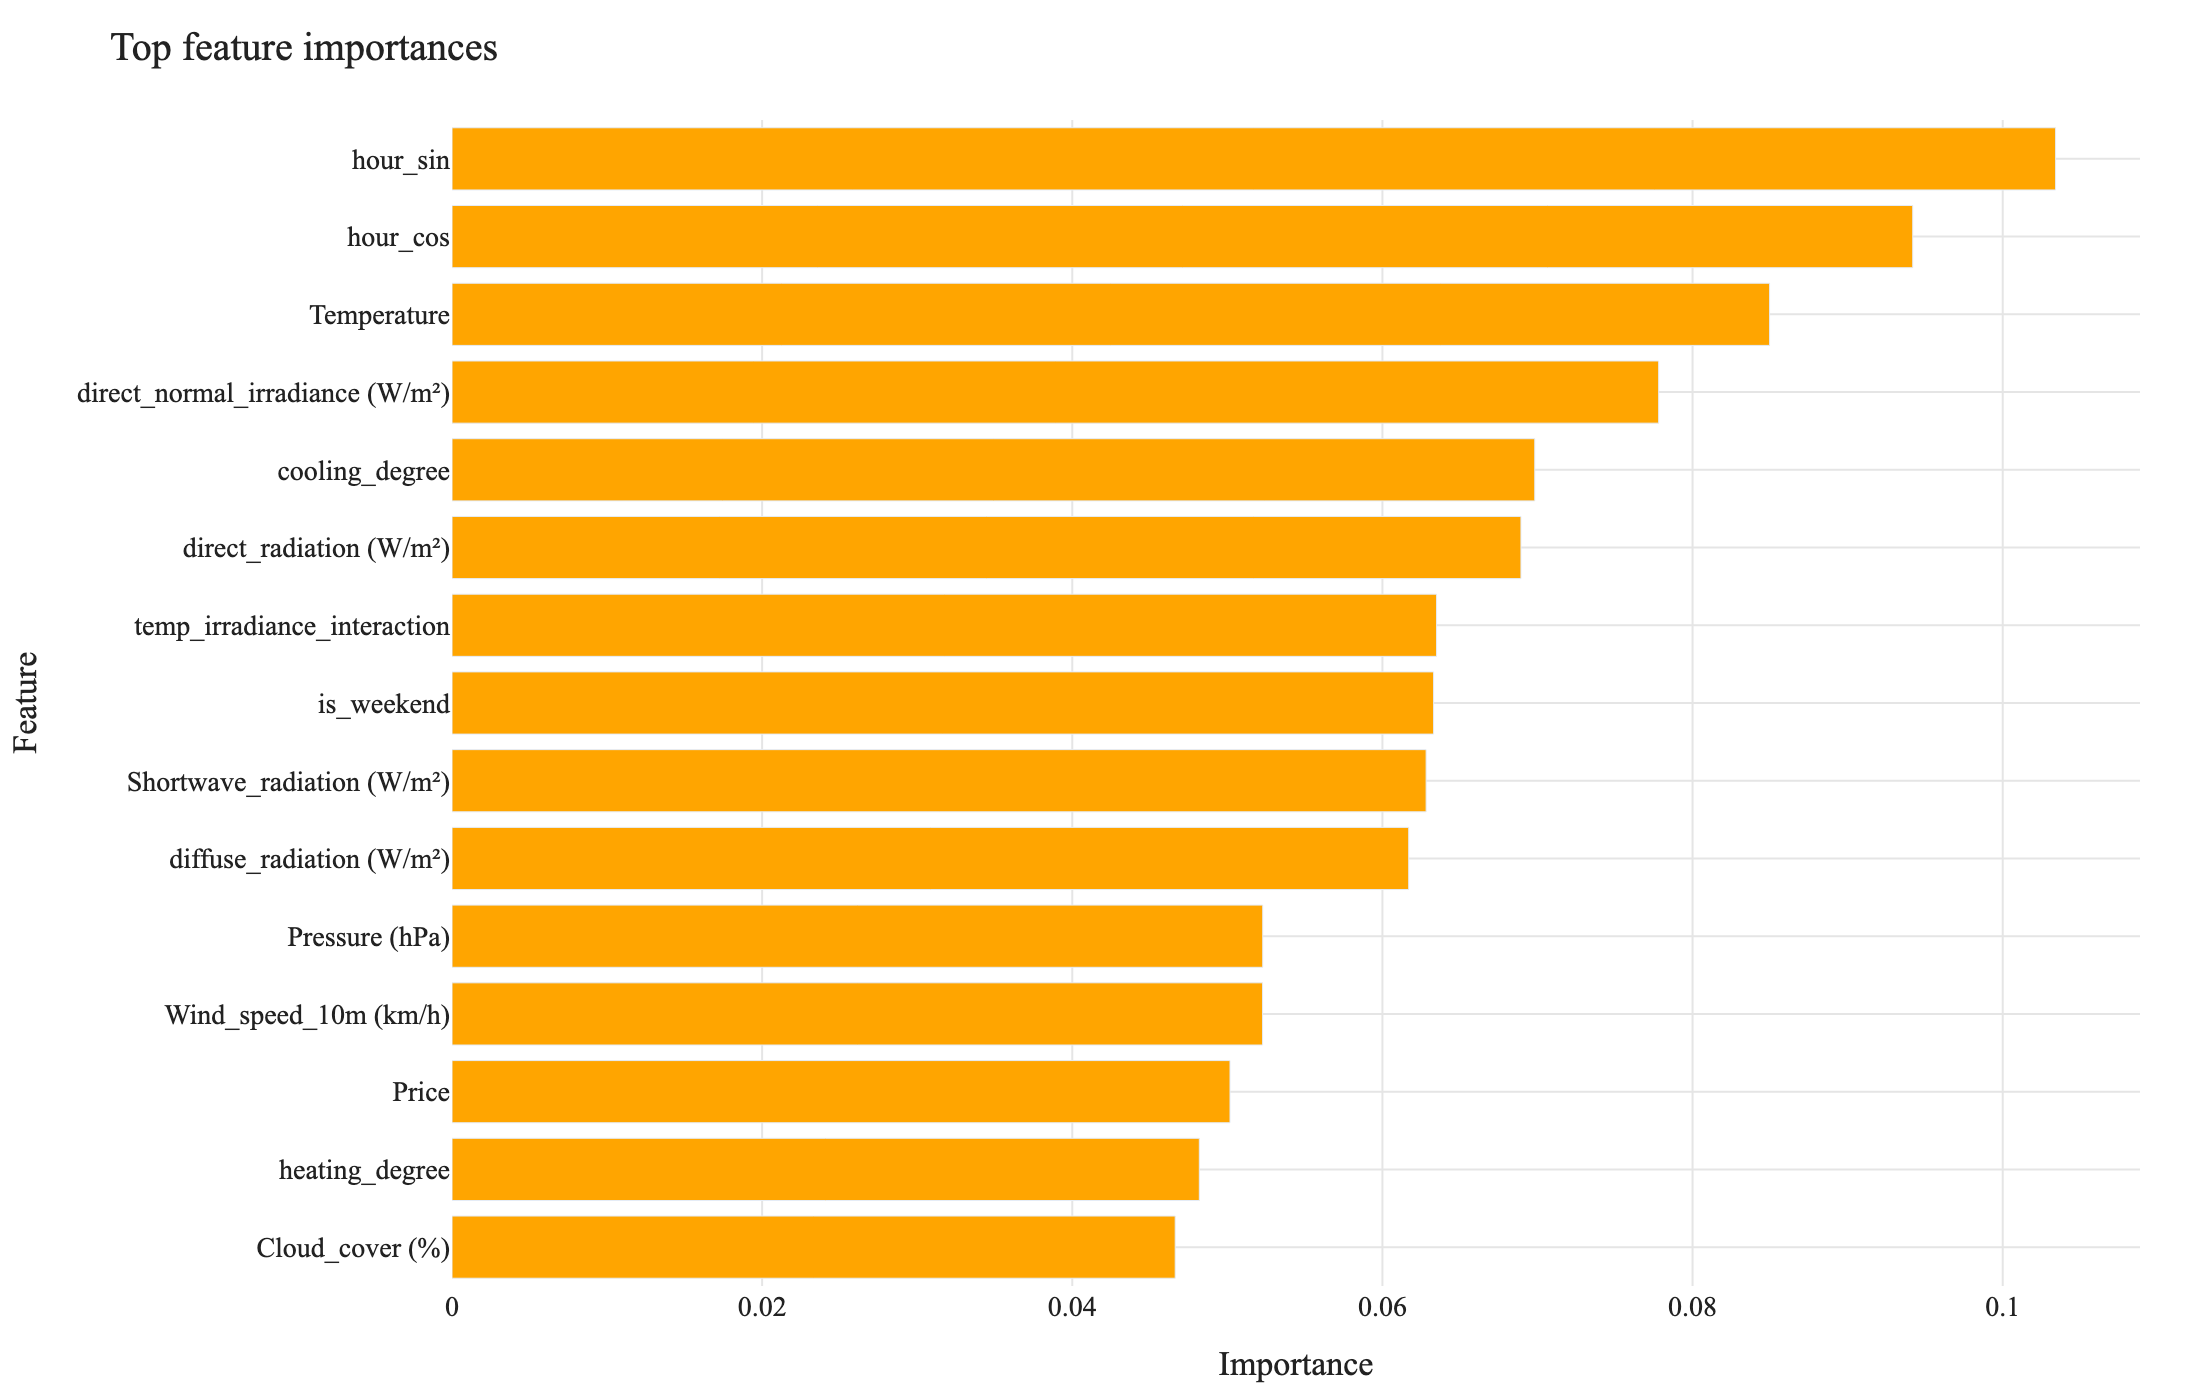
\includegraphics[width=0.95\linewidth]{figures/ml_feat_importance.png}
  \caption{Feature-Importance (modellbasiert, z.\,B. Random Forest). Zeitliche Marker (Hour, Day) und Wetter (Temperature/PV) dominieren, Lags tragen Persistenzinformation.}
  \label{fig:fe_importance}
\end{figure}

\subsection*{5.5 Summary}
Feature Engineering hat den Datensatz f{"u}r statistische Modelle (ARIMA, STL-basiert) und ML-Modelle (GBM, RF) aufbereitet: Diurnalit{"a}t und Wocheneffekte sind explizit, Persistenz wird durch Lags/Rolling-Stats abgebildet, Wetter- und Interaktionsmerkmale erfassen nichtlineare Treiber. Reproduzierbarkeit wird durch skriptbasierte Generierung (Notebook/`src/features.py`) und Versionierung der Feature-Schemata sichergestellt. Validierung erfolgt {\"u}ber Cross-Validation/WFA sowie Drift-Monitoring der Merkmalverteilungen. Gute Praktiken folgen \cite{Zheng2020,Hyndman2021}.

\printbibliography

\end{document}
